%%%%%%%%%%%%%%%%%%%%%%%%%%%%%%%%%%%%%%%%%
% Beamer Presentation
% LaTeX Template
% Version 1.0 (10/11/12)
%
% This template has been downloaded from:
% http://www.LaTeXTemplates.com
%
% License:
% CC BY-NC-SA 3.0 (http://creativecommons.org/licenses/by-nc-sa/3.0/)
%
%%%%%%%%%%%%%%%%%%%%%%%%%%%%


%----------------------------------------------------------------------------------------
%	PACKAGES AND THEMES
%----------------------------------------------------------------------------------------

%\documentclass[10pt]{beamer}
\documentclass[]{beamer}



\DeclareMathOperator*{\argmin}{arg\,min}


%%%%%%%%%%%%%

\usepackage{hyperref}


\newcommand{\bi}{\begin{itemize}}
\newcommand{\ei}{\end{itemize}}
\newcommand{\m}{\item}
\newcommand{\be}{\begin{enumerate}}
\newcommand{\ee}{\end{enumerate}}
\newcommand{\al}{\alert}
\newcommand{\ul}{\underline}


\mode<presentation> {

% The Beamer class comes with a number of default slide themes
% which change the colors and layouts of slides. Below this is a list
% of all the themes, uncomment each in turn to see what they look like.

%\usetheme{default}
%\usetheme{AnnArbor}
%\usetheme{Antibes}
%\usetheme{Bergen}
%\usetheme{Berkeley}
%\usetheme{Berlin}
%\usetheme{Boadilla}
%\usetheme{CambridgeUS}
%\usetheme{Copenhagen}
%\usetheme{Darmstadt}
%\usetheme{Dresden}
\usetheme{Frankfurt}
%\usetheme{Goettingen}
%\usetheme{Hannover}
%\usetheme{Ilmenau}
%\usetheme{JuanLesPins}
%\usetheme{Luebeck}
%\usetheme{Madrid}
%\usetheme{Malmoe}
%\usetheme{Marburg}
%\usetheme{Montpellier}
%\usetheme{PaloAlto}
%\usetheme{Pittsburgh}
%\usetheme{Rochester}
%\usetheme{Singapore}
%\usetheme{Szeged}
%\usetheme{Warsaw}

% As well as themes, the Beamer class has a number of color themes
% for any slide theme. Uncomment each of these in turn to see how it
% changes the colors of your current slide theme.

%\usecolortheme{albatross}
%\usecolortheme{beaver}
%\usecolortheme{beetle}
%\usecolortheme{crane}
%\usecolortheme{dolphin}
%\usecolortheme{dove}
%\usecolortheme{fly}
%\usecolortheme{lily}
%\usecolortheme{orchid}
%\usecolortheme{rose}
%\usecolortheme{seagull}
%\usecolortheme{seahorse}
%\usecolortheme{whale}
%\usecolortheme{wolverine}

%\setbeamertemplate{footline} % To remove the footer line in all slides uncomment this line
%\setbeamertemplate{footline}[page number] % To replace the footer line in all slides with a simple slide count uncomment this line

%\setbeamertemplate{navigation symbols}{} % To remove the navigation symbols from the bottom of all slides uncomment this line
}


%\setbeamertemplate{headline}
%{%
% \begin{beamercolorbox}{section in head/foot}
%\vskip1pt\insertnavigation{\textwidth}{}{}\vskip2pt
%  \end{beamercolorbox}
%}

\setbeamercolor{section in head/foot}{bg=lightgray} %set the top navigation bar background color
\setbeamertemplate{footline}[frame number] % set frame page number only
\usepackage{appendixnumberbeamer} % total will not include appendix frame numbers 

\beamertemplatenavigationsymbolsempty



\usepackage{graphicx} % Allows including images
% graphicx also allows for resizebox
% graphicx also allows for \scalebox
\usepackage{caption}
\usepackage{subcaption} % packgage for subcaption in subfigures
% The subfig and subcaption packages can not be used in cooperation with each other. Instead, you can usecaption package with subfig to add some flavor to the captions and subcaptions
\usepackage{bm} % make bold math symbols
\usefonttheme{professionalfonts}
%\usepackage{newtxtext,newtxmath} % for professional fond to load a Times Roman clone
\usepackage{tabularx} % extra features for tabular environment
\usepackage{booktabs} % Allows the use of \toprule, \midrule and \bottomrule in tables
\usepackage{adjustbox} % allows adjustbox
\usepackage{amsmath}  
\usepackage{amsfonts}
\usepackage{hyperref} % package for hyper link

% the following hypersetup makes link blue
\hypersetup{
  colorlinks   = true, %Colours links instead of ugly boxes
  urlcolor     = blue, %Colour for external hyperlinks
  linkcolor    = blue, %Colour of internal links
  citecolor   = blue %Colour of citations
}


\usepackage{float} % make the table H effective
\restylefloat{table}
\usepackage{color, colortbl}
\usepackage{booktabs} % package for tex professional table
\usepackage{mathtools} % package for \coloneqq
\usepackage{multirow} % multirow for intuition page.

% make pdf dark mode
%\usepackage{xcolor}
%\pagecolor[rgb]{0,0,0} %black
%\color[rgb]{0.5,0.5,0.5} %grey

\usepackage{pifont}% http://ctan.org/pkg/pifont
\newcommand{\cmark}{\ding{51}}%
\newcommand{\xmark}{\ding{55}}%



\usepackage{tikz} % graph in latex
\usetikzlibrary{positioning,arrows.meta} %tikz diagram
\usepackage{pgfplots}
\pgfplotsset{compat=newest} %this setting allow node to go to the correct place
\usepgfplotslibrary{fillbetween}

% use the tikz external library to cache tikz drawings
\usetikzlibrary{external}
\tikzexternalize[prefix=tikz/,optimize command away=\includepdf]


%\bibliography{bibliography}
%\usepackage[american]{babel}
%\usepackage{csquotes}
%\usepackage[style=apa]{biblatex}
%\DeclareLanguageMapping{american}{american-apa}
%\addbibresource{References.bib}

\usepackage{natbib} % package for citation


%\usepackage{subfigure} % subfigure package
%\captionsetup[subfigure]{labelformat=empty}
% The subfig and subcaption packages can not be used in cooperation with each other. Instead, you can usecaption package with subfig to add some flavor to the captions and subcaptions

%\usepackage{natbib} % package for citation

% define a comment line that does nothing to hide content
\newcommand{\comment}[1]{}
\newcommand{\lnb}[1]{%
  \ln\left(#1\right)%
}
\renewcommand{\baselinestretch}{1.0} %  scales the default interline space to 1.0 its default value. 

% define a comment that can scale the equation 
\newcommand\scalemath[2]{\scalebox{#1}{\mbox{\ensuremath{\displaystyle #2}}}}

%----------------------------------------------------------------------------------------
%	TITLE PAGE
%----------------------------------------------------------------------------------------

\title[Decentralized Finance]{\huge{Decentralized Finance} \\
\vspace{6mm}
\small{MGT 4074 Fintech \& Crypto Tokens, Section A, Spring 2025}
} % The short title appears at the bottom of every slide, the full title is only on the title page


%\subtitle{Presentation to Shanghai International Studies University}


\author[Joseph Hall]{Joseph Hall} % Your name
\institute[GT]{Georgia Institute of Technology} % Your institution as it will appear on the bottom of every slide, may be shorthand to save space
 % Your institution for the title page
 % Your email address
 
\date{September 29, 2025} 
 % Date, can be changed to a custom date if without date



%---------------------------------------------------------------------------
\begin{document}

\newcolumntype{d}[1]{D{.}{.}{#1}}


\begin{frame}
\titlepage % Print the title page as the first slide
\end{frame}


%----------------------------------------------------------------------------------------

%	PRESENTATION SLIDES
%----------------------------------------------------------------------------------------

%-----------------------------------------------



%---------------------------------------------------------------------
%---------------------------------------------------------------------
%\section*{Introduction}
% When I comment the introduction section, fewer sections show up in navigation
%---------------------------------------------------------------------
%---------------------------------------------------------------------



\begin{frame}{Welcome! Today is Monday 9/29/25}

\begin{center}

Thank you for submitting Homework \#2. \\ 

For Wednesday: Please read: \\ 
    \href{https://medium.com/@marthe_naudts/highly-profitable-trading-strategies-avraham-eisenberg-and-the-legalities-and-ethics-of-crypto-6bd81ef1caf9}{``Don't Trust, Verify'' }\\ 
    by Marthe Naudts on Medium 
\end{center}

\end{frame}

\begin{frame}{Verification of Completion for HW2}

\bi 
\m Anyone with an internet connection can verify that \emph{someone} did your homework
\m Anyone (e.g. Nnadozie and me) who knows the mapping of wallets to names can verify who 
\ei 
\vfill 

\begin{center}
   \href{https://sepolia.etherscan.io/address/0x41c8826d7c4b54f961cc14bd22ca0abd398073f6}{The contract} 
    \vfill \href{https://sepolia.etherscan.io/token/0x41c8826d7c4b54f961cc14bd22ca0abd398073f6}{The token}
\end{center}
\vfill 
    
\end{frame}

\begin{frame}{In the News: Economists Remain Crypto Bears}

\begin{center}
    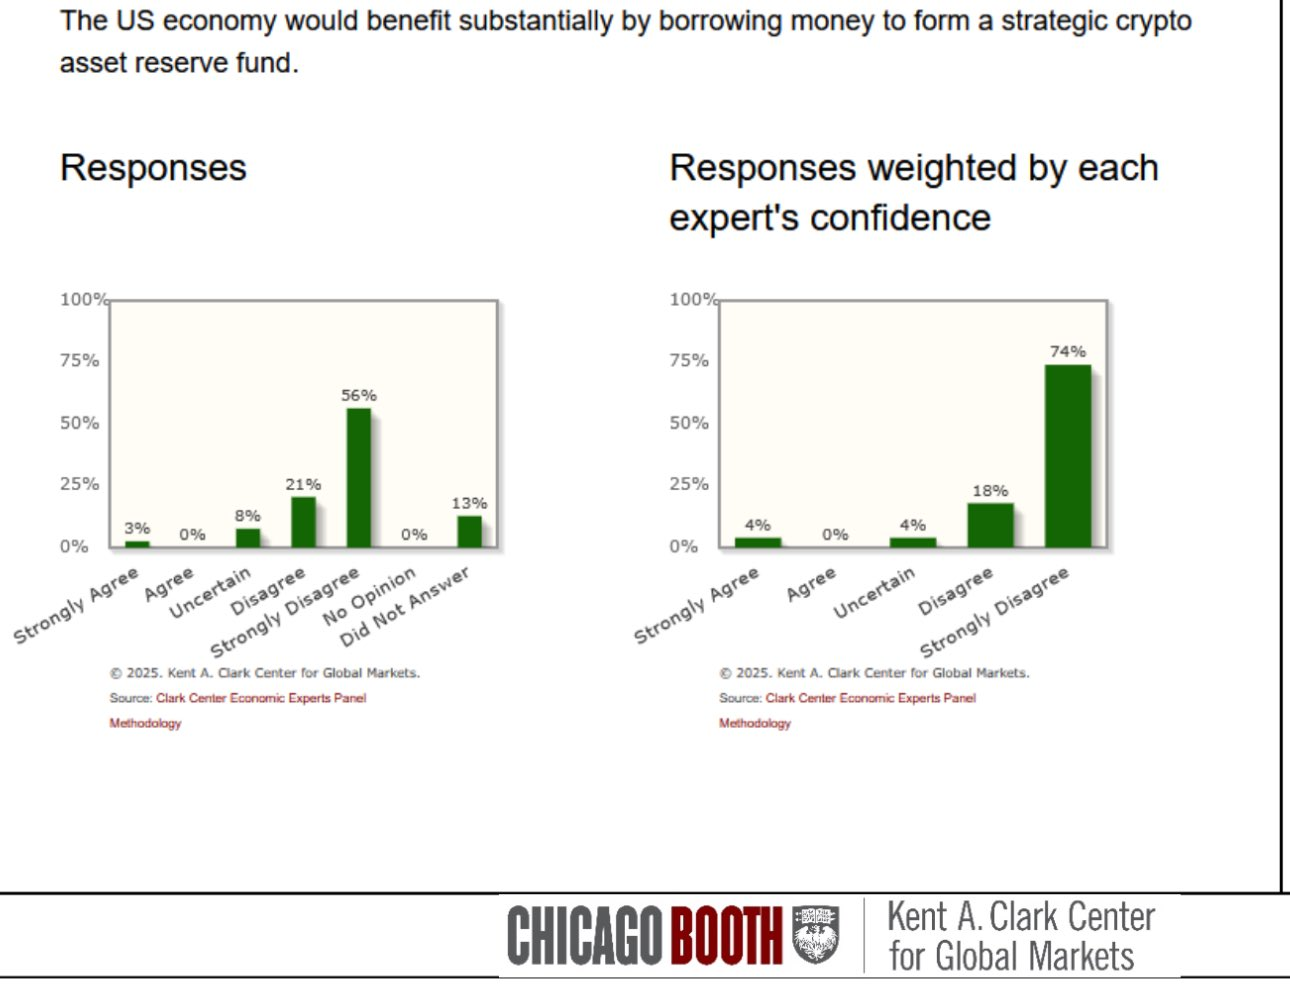
\includegraphics[width = 0.75\textwidth]{booth_survey.jpeg}
\end{center}

2013 Nobel Laureate Eugene Fama: Crypto ``will go to zero within 10 years''. 
    
\end{frame}

\begin{frame}{In the News: CFPB to Pause All Enforcement}

\begin{center}
    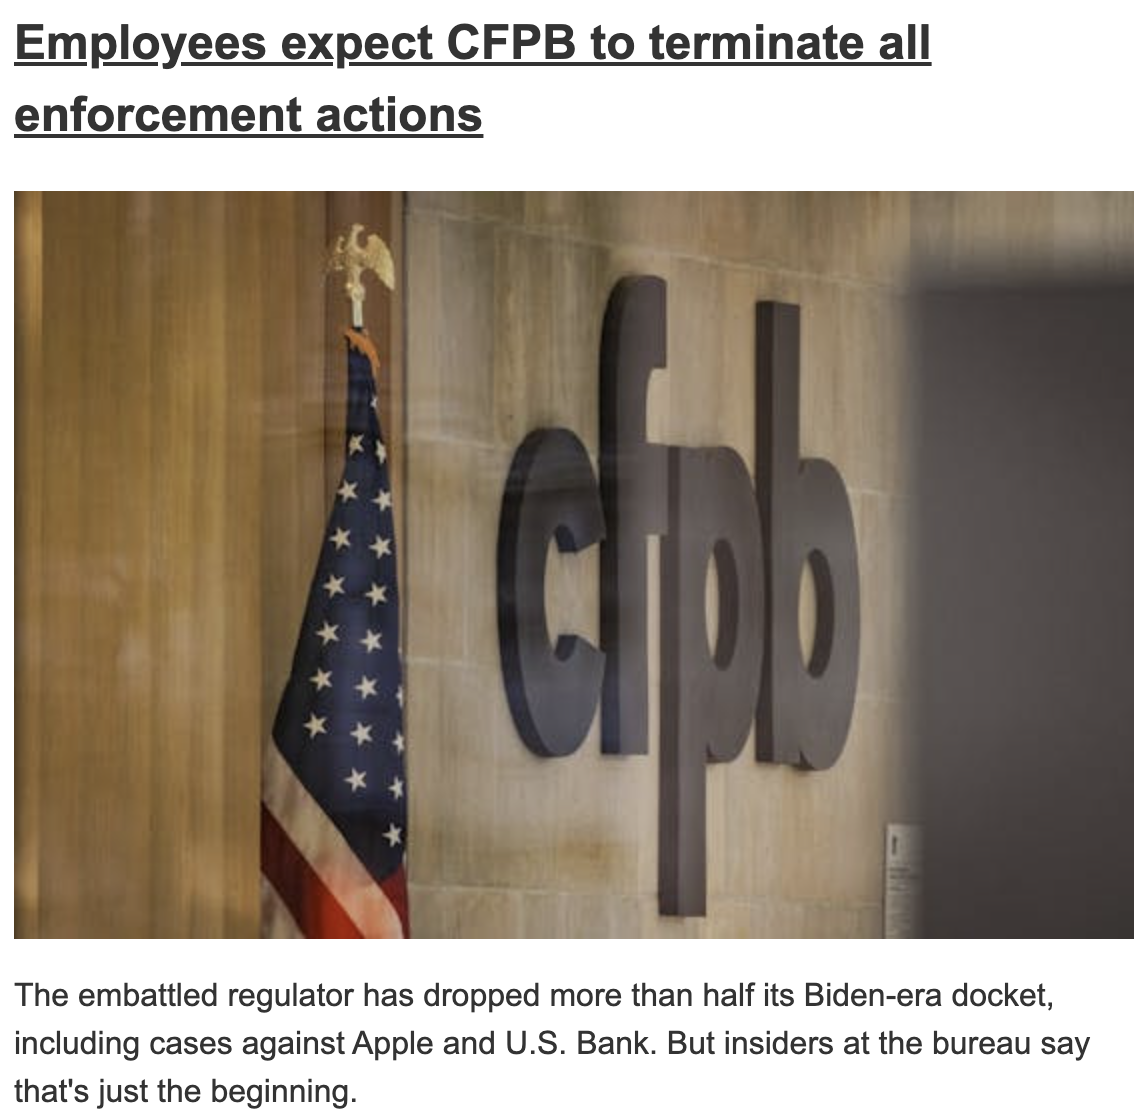
\includegraphics[height = .9\textheight]{cfpb.png}
\end{center}
    
\end{frame}

\begin{frame}{In the News: Downward Trend in Crypto Payments}

From \href{https://www.kansascityfed.org/documents/11707/PaymentsSystemResearchBriefing25HayashiRouth0924.pdf}{Hayashi \& Routh:}

\begin{center}
    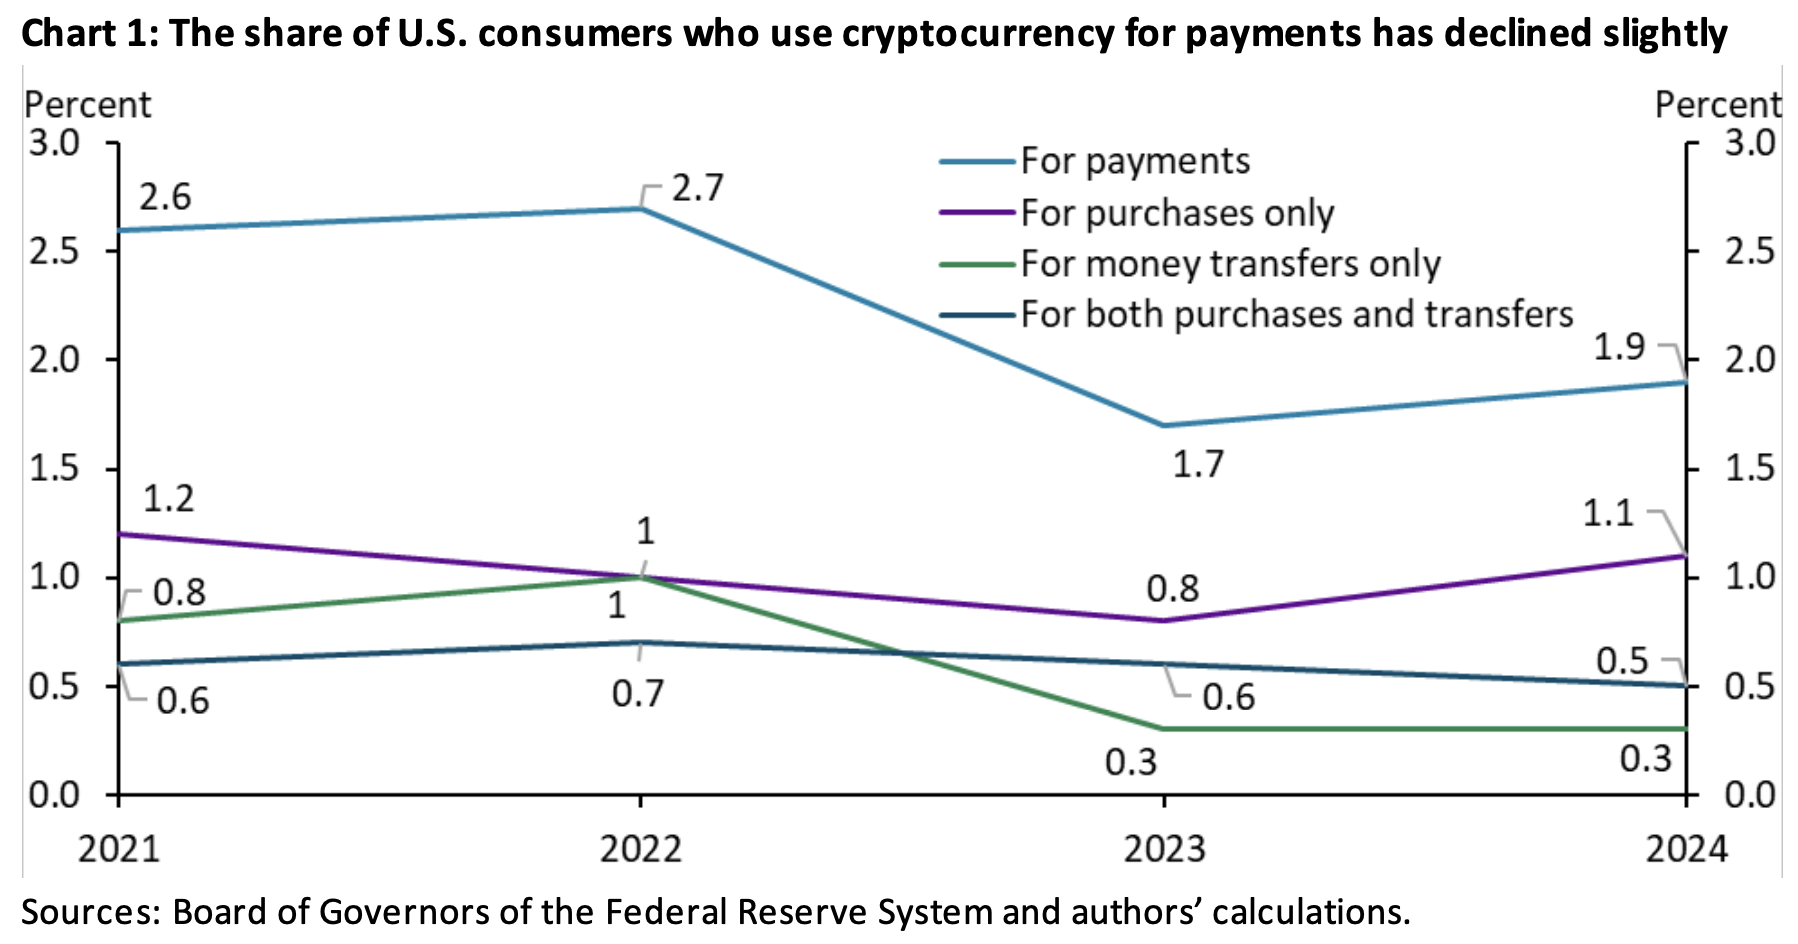
\includegraphics[width = .9\textwidth]{kcfed.png}
\end{center}

\end{frame}

\begin{frame}{Matt Levine's Commentary}

``I suppose it is often the case that a technology is introduced with great hype to solve one particular problem, and then turns out to be more or less irrelevant to that problem but quite useful for some other problem. Here Bitcoin was introduced to allow for peer-to-peer permissionless payments, for which it has turned out to be a dud. But Bitcoin is very good at an unrelated thing, which is “going up in price.” (You can see why that would make it bad as a payments medium!) So it has caught on and become widely adopted, even though its original premise was kind of wrong.''

\end{frame}

\begin{frame}{Matt Levine's Commentary, Contd.}
    
``Incidentally the point of that Kansas City Fed research note appears to be to express skepticism about stablecoins as a payments mechanism, in the face of growing optimism elsewhere. I don’t know if that follows. Crypto is not widely used for payments for a number of reasons, including (1) prices are volatile, (2) you can’t reverse payments and (3) you can’t send crypto from your bank’s app. Stablecoins fix the first problem and, with a certain amount of pushing to become part of the financial mainstream, could solve the other two as well.''
    
\end{frame}


\begin{frame}{Backtracking: Bremmerman's Limit}

In our unit on Cryptography and Blockchains, I forgot to mention the very important \textbf{Bremmerman's Limit}. \\ \vfill 

Bremmerman's Limit gives an upper bound to computation speed in the physical universe. It is \textbf{$1.4\times 10^{50}$ bits per second per kilogram}. \\ \vfill 

A Bremmerman computer the mass of Earth could theoretically crack a 256-bit hash in about 2 minutes, or a 512-bit hash in $10^{75}$ years. \\ \vfill 

Problems which require more than $10^{93}$ bits of computation are called \textbf{transcomputational}, meaning a Bremmerman computer the size of Earth would not solve the problem within the current estimated age of Earth. \\ \vfill 

In practice, of course, engineering considerations restrict feasible computers far, far below this limit. Suffice it to say, your on-chain assets are safe from a brute force attack for the forseeable future. 
    
\end{frame}


\begin{frame}
\frametitle{Roadmap}
\tableofcontents
\end{frame}

%------------------------------------------------

%------------------------------------------------
% insert table of content before each section or subsection
%------------------------------------------------
\AtBeginSection[]
%\AtBeginSubsection[]
{
\begin{frame}
\frametitle{Roadmap}
\tableofcontents[currentsection,currentsubsection]
%\tableofcontents[currentsection]
\end{frame}
}
%------------------------------------------------





\section{Pain Points of TradFi}


\begin{frame}
\frametitle{The Traditional Financial System}

\bi
\m The traditional financial system allows people and institutions to trade \ul{time} and \ul{risk}, using \ul{promises}
\m The purpose of the system is to enable agents to \ul{smooth consumption} and \ul{share risk}
\bi \pause
\m Essential functions for a society!
\m When thinking about defi, remember the purpose of finance!
\ei \pause
\m But not all is good with tradfi:
\bi
\m Complexity
\m Rents
\m Justice
\m Access
\ei
\ei

\end{frame}

%\subsection{Complexity}

\begin{frame}
\frametitle{A Promise in Tradfi}

\begin{center}
\includegraphics<1>[width = 0.9\textwidth]{pics/isda1.png}
%\includegraphics<2>[width = 0.9\textwidth]{pics/isda1point5.png}
\includegraphics<2>[width = 0.5\textwidth]{pics/isda2.png}
\includegraphics<3>[width = 0.5\textwidth]{pics/isda3.png}
\includegraphics<4>[width = 0.5\textwidth]{pics/isda4.png}
\includegraphics<5>[width = 0.5\textwidth]{pics/isda5.png}
\includegraphics<6>[width = 0.45\textwidth]{pics/isda6.png}
\end{center}

\vspace{1ex}

\href{https://www.gbm.hsbc.com/financial-regulation/2002-isda-master-agreement}{Source}

\end{frame}

%\subsection{Rents}


\begin{frame}
\frametitle{Rents}

\begin{center}
\includegraphics<1>[width = 0.8\textwidth]{pics/creditcards.png}
\end{center}

\vspace{2ex}
\footnotesize

\href{https://www.fool.com/the-ascent/research/average-credit-card-processing-fees-costs-america/}{Source}

In Economics, a \textbf{rent} is any recurring payment earned in excess of the cost to provide it. Persistent rents are evidence of \textbf{barriers to entry} or other impediments to perfect competition. 

\end{frame}


\begin{frame}
\frametitle{Finance in the USA}

\begin{center}
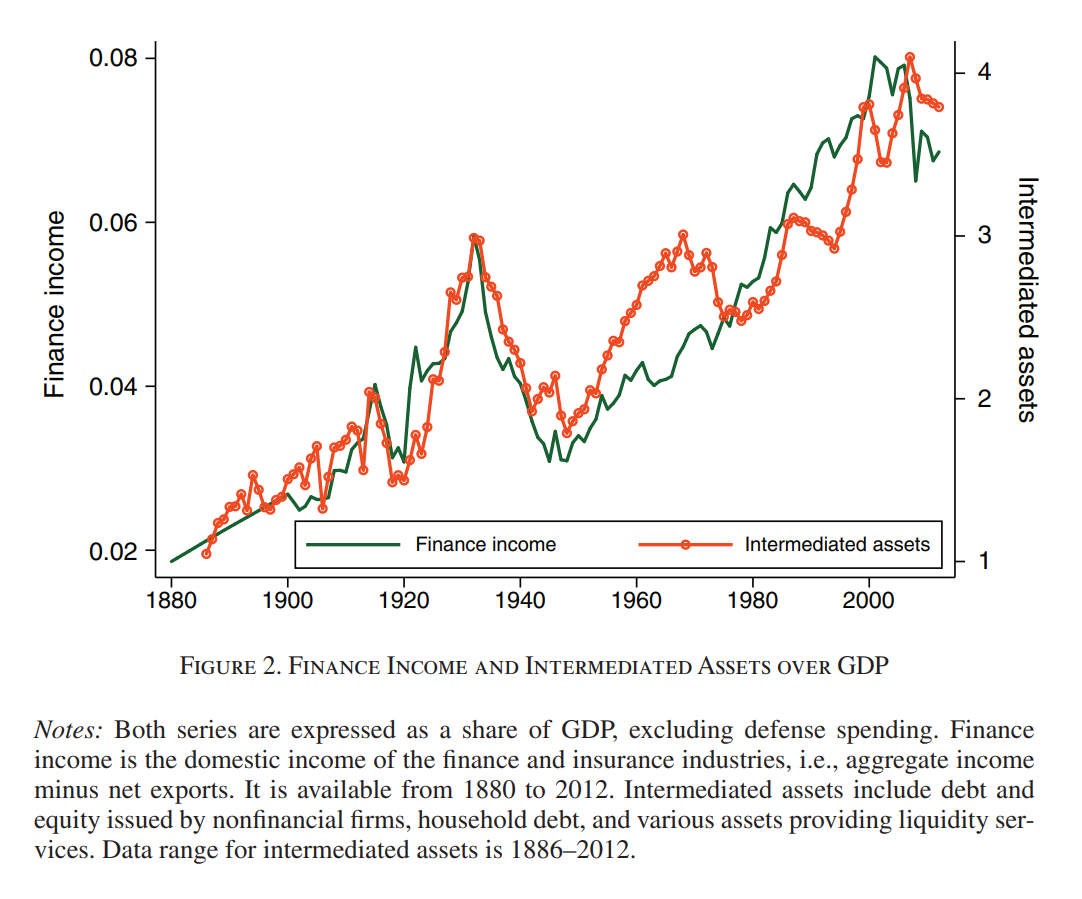
\includegraphics[width = 0.7\textwidth]{pics/philippon.png}
\end{center}
\footnotesize

(\href{https://www.aeaweb.org/articles?id=10.1257/aer.20120578}{Philippon (2015)}.) Are we getting 4x better value per GDP from the financial services industry than in 1880? 

\end{frame}

\begin{frame}
\frametitle{Will innovations like Venmo fix this?}


\begin{center}
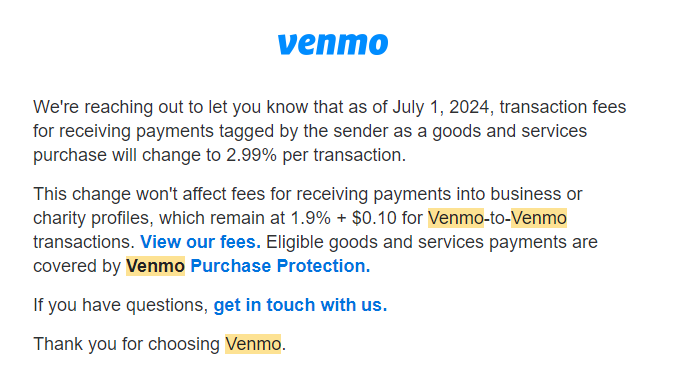
\includegraphics[width = 0.8\textwidth]{venmo2.png}
\end{center}

\vspace{2ex}
\footnotesize

\href{https://twitter.com/AnthonyLeeZhang/status/1407551975684775943/photo/1}{Source}

\end{frame}


\begin{frame}
\frametitle{Will Venmo fix this?}


\begin{center}
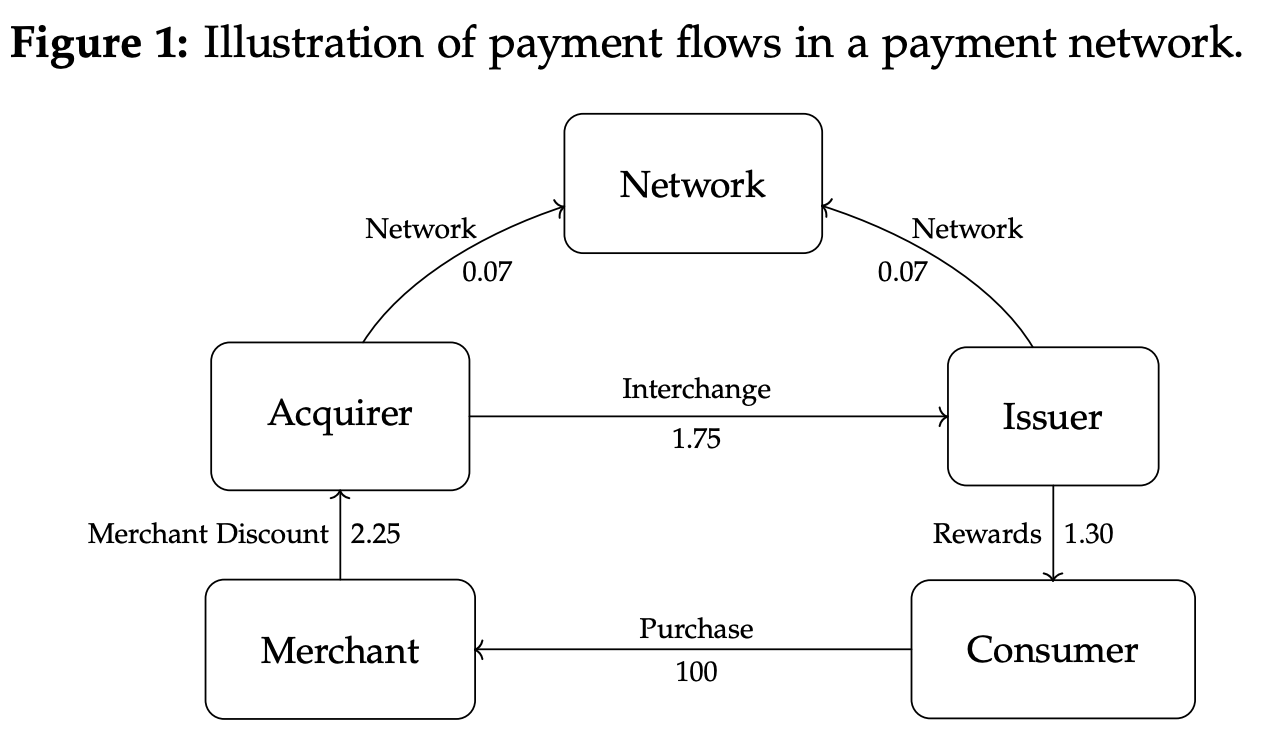
\includegraphics[width = 0.8\textwidth]{paymet_flows.png}
\end{center}

\end{frame}

\begin{frame}{Will Venmo fix this?}

``This paper compares the relative merits of regulating prices versus increasing competition in U.S. payment markets ... merchants in the U.S. typically charge consumers the same price for different payment methods ... \textbf{Price coherence} incentivizes networks to charge high merchant fees to fund consumer rewards ... High credit card rewards inflate retail prices for all consumers while encouraging excessive credit card use ... There are large gains from either capping credit card merchant fees or uncapping debit card merchant fees, whereas encouraging competition is harmful [because it will re-create the forces that caused over-use of credit cards].'' 
\flushright \href{https://luluywang.github.io/PaperRepository/payment_jmp.pdf}{Wang (2024)} says \ul{No} (do we agree?) 
    
\end{frame}

%\subsection{Justice}


\begin{frame}
\frametitle{Justice?}

\begin{center}
\includegraphics<1>[width = 0.5\textwidth]{pics/canadatruckers.png}
\includegraphics<2>[width = 0.35\textwidth]{pics/paypal.jpg}
\end{center}

\vspace{2ex}
\footnotesize

\href{https://www.businessinsider.com/trudeau-canada-freeze-bank-accounts-freedom-convoy-truckers-2022-2}{Source 1} and \href{https://www.paypalobjects.com/marketing/ua/pdf/US/en/acceptableuse-full-110322.pdf}{source 2}

\end{frame}

%\subsection{Access}


\begin{frame}
\frametitle{Access}

\begin{center}
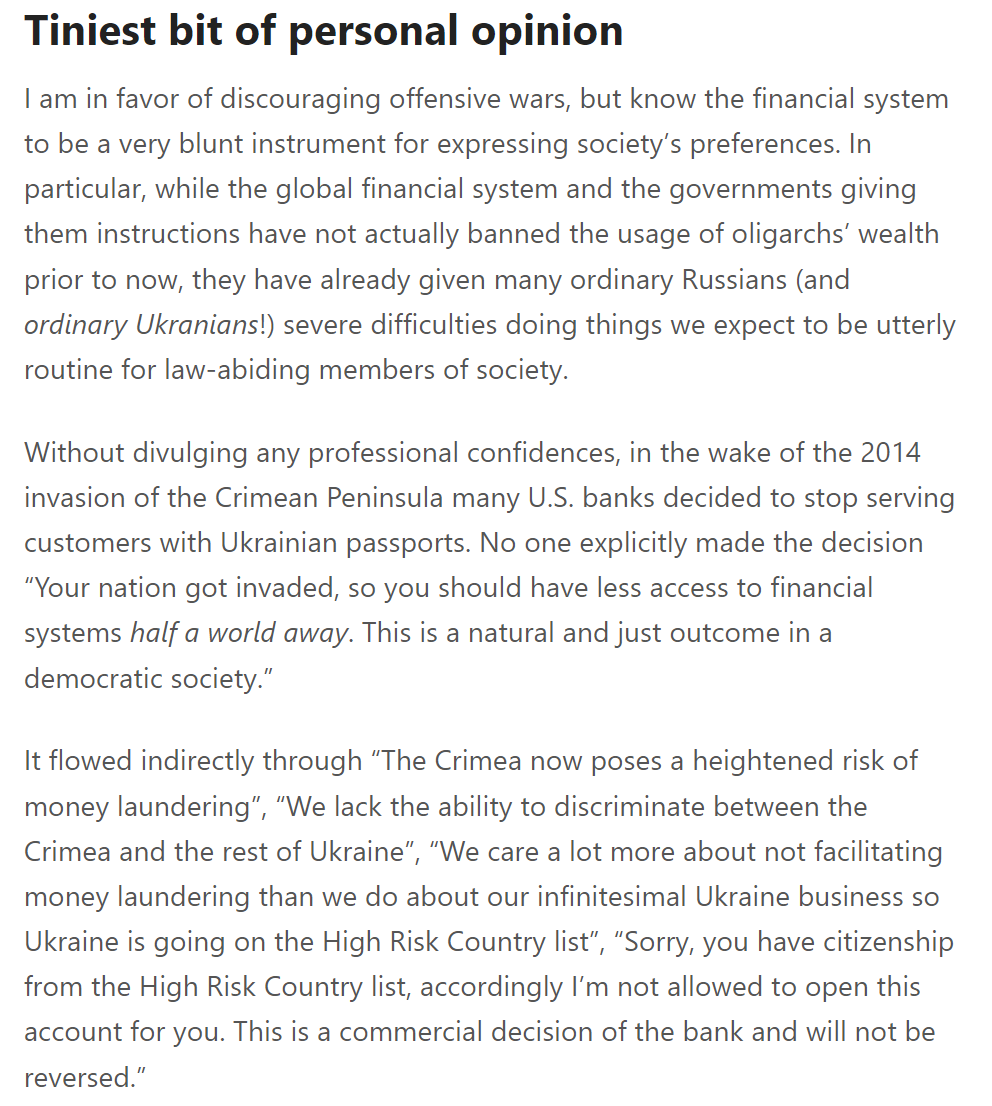
\includegraphics[width = 0.55\textwidth]{pics/bitsaboutmoney.png}
\end{center}

Source: \href{https://bam.kalzumeus.com/archive/moving-money-internationally/}{Bits About Money} on international transfers
\end{frame}

\begin{frame}
\frametitle{Other Issues with Tradfi}

\bi
\m High entry costs, low competition 
\m Out-dated infrastructure, lack of composability
\m Crashes, fragility, systemic risk
\m Opacity, politicization 
\ei
\end{frame}


\section{Promise of DeFi}


\begin{frame}
\frametitle{Decentralized Finance: The Vision}

\bi
\m Simple,
\m Low-cost and competitive,
\m Just and non-discretionary,
\m Accessible,
\m Always at the technological frontier, 
\m Transparent, and 
\m Trustlessly safe by design 
\ei

\end{frame}


\begin{frame}
\frametitle{DeFi has leveled off at $\sim\$100$B}

\begin{center}
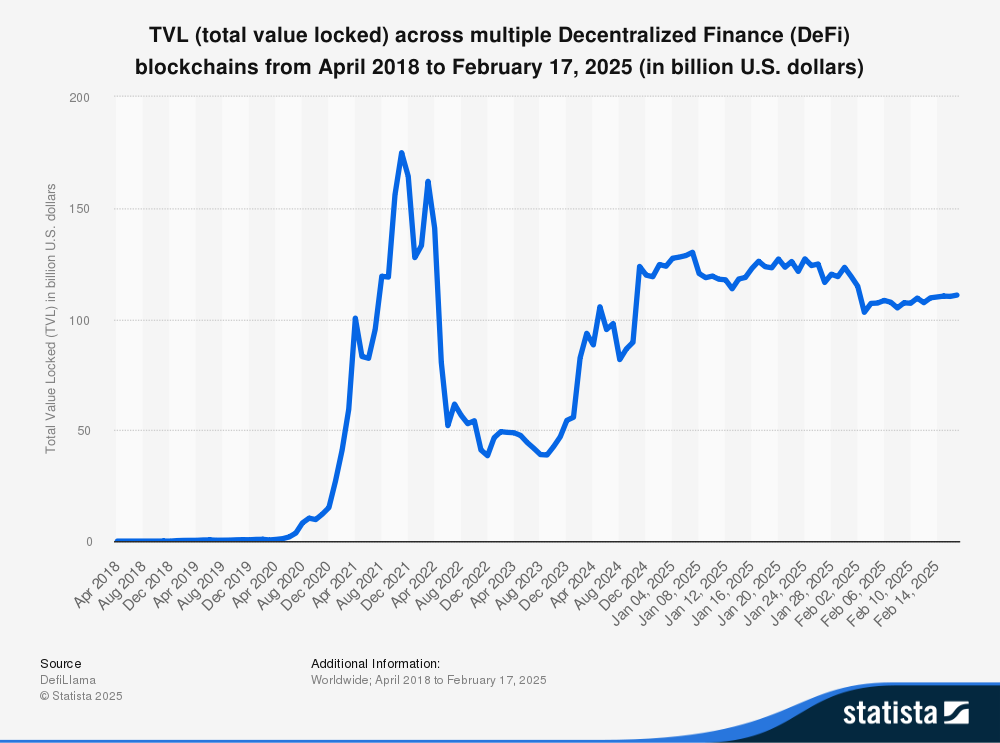
\includegraphics[width = 0.8\textwidth]{statistia.png}
\end{center}

\href{https://www.statista.com/statistics/1272181/defi-tvl-in-multiple-blockchains/}{Source}

\end{frame}

\begin{frame}
\frametitle{But remains small compared to TradFi\ldots}

\begin{center}
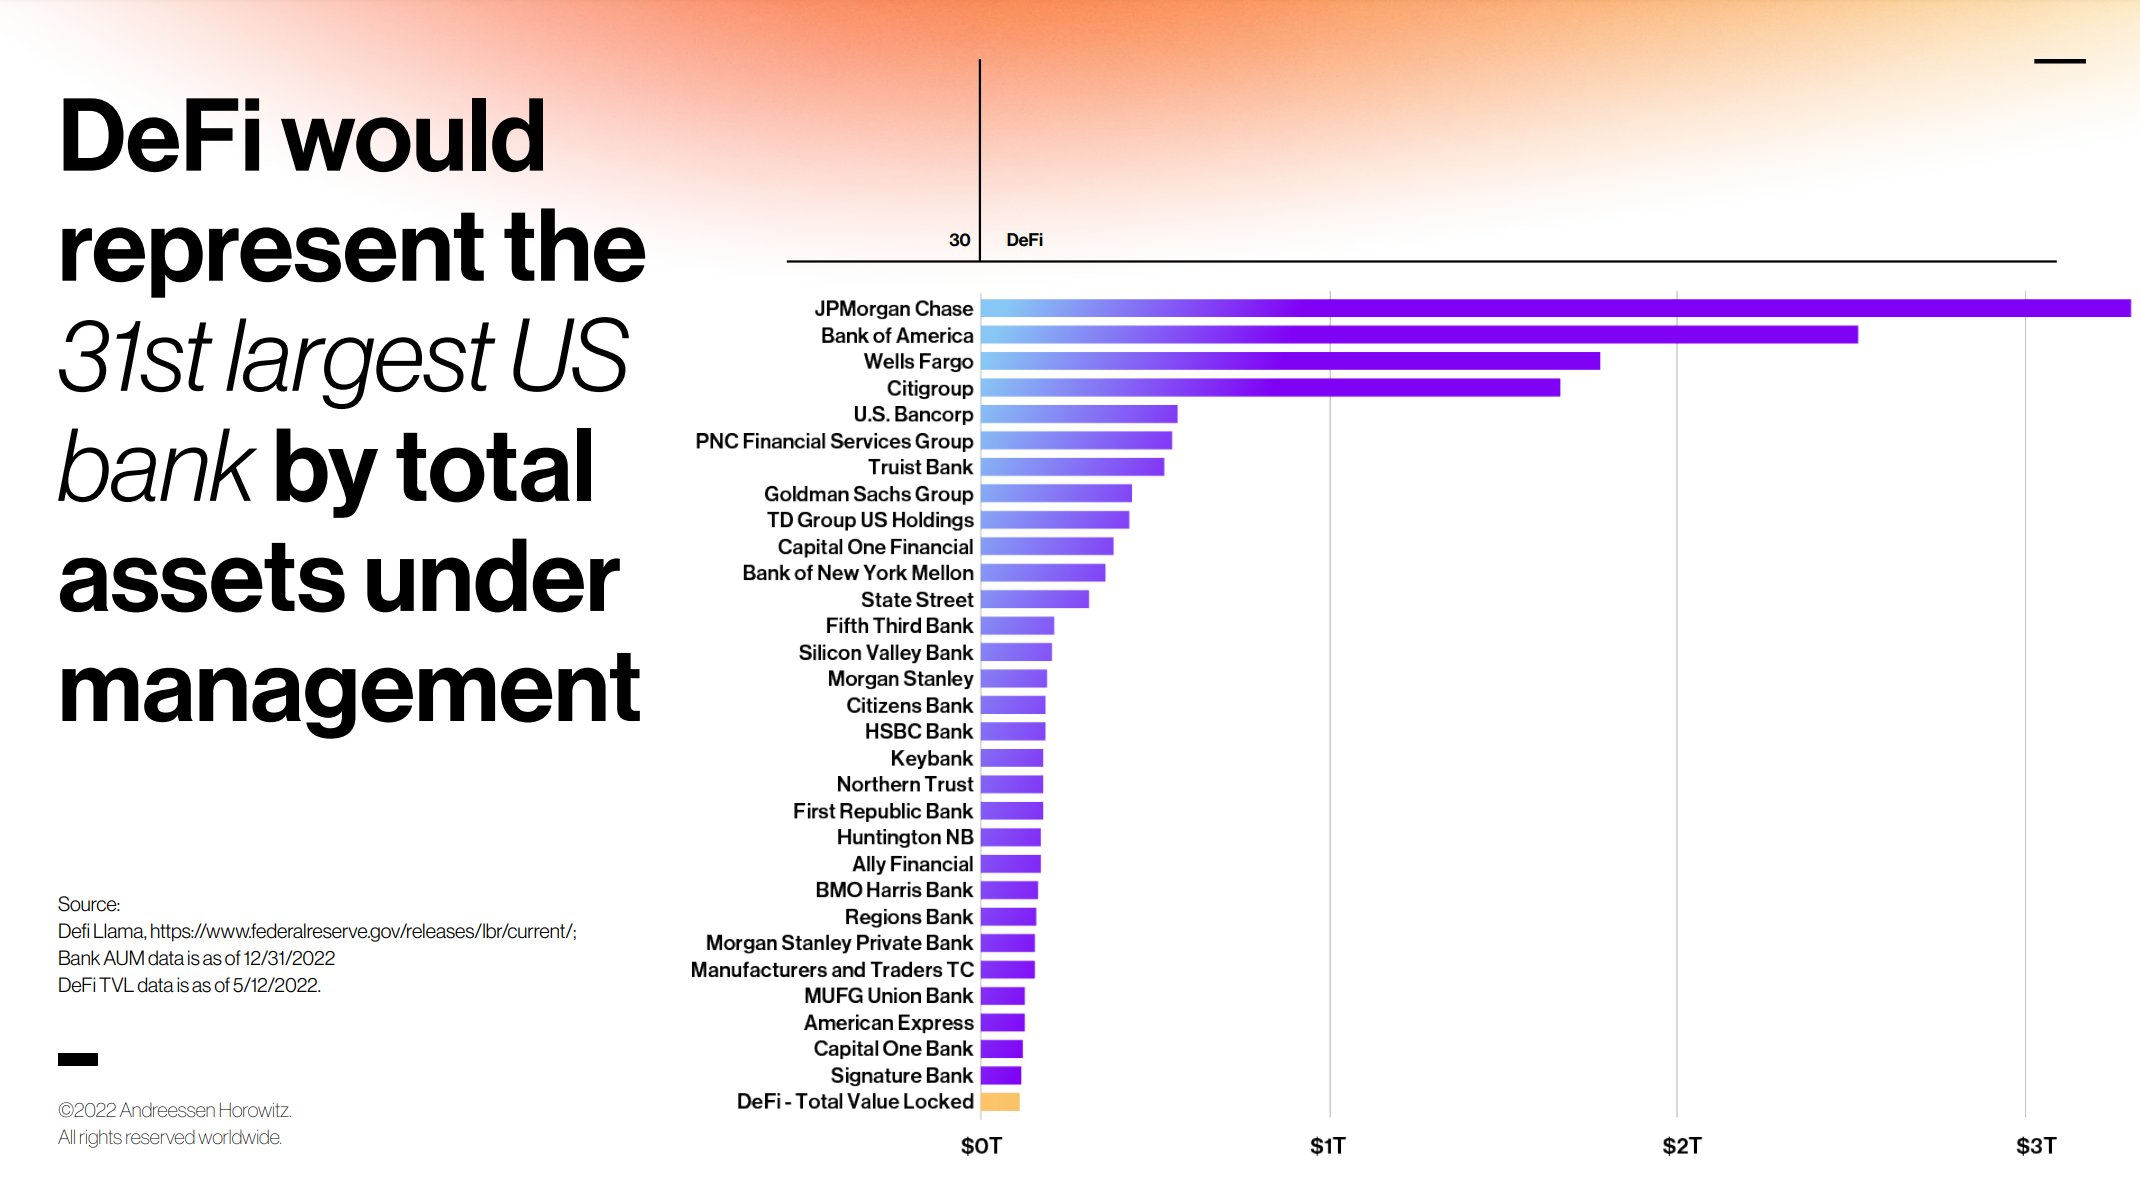
\includegraphics[width = 0.8\textwidth]{pics/defitvlbanks.jpg}
\end{center}

\vspace{2ex}
\footnotesize

\href{https://twitter.com/AnthonyLeeZhang/status/1564372656610230279/photo/1}{Source}

\end{frame}


\begin{frame}
\frametitle{Defi Contracts\ldots}

\begin{center}
\includegraphics<1>[width = 0.9\textwidth]{pics/unicode1.png}
\includegraphics<2>[width = 0.9\textwidth]{pics/unicode2.png}
\includegraphics<3>[width = 0.6\textwidth]{pics/unicode3.png}
\end{center}

\href{https://github.com/Uniswap}{Source}

\end{frame}

\begin{frame}{Critical questions for DeFi}

\bi
\m What is the classic finance question being solved?
\m How does the structure of blockchain tech influence the answer? \pause
\m What weaknesses of tradfi do these applications address and improve on?
\m What new weaknesses are introduced? \pause
\m What kinds of \textbf{promises} that couldn't be made, now can be made, thanks to blockchain technology?
\ei

\end{frame}





\begin{frame}
\frametitle{Proof of Stake}

\bi
\m Originally, ETH mining proof-of-work, similar to BTC
\m On Sept 15 2022, ETH switched to \ul{proof of stake} -- called \textbf{``The Merge''}
\m Reduced energy consumption by \textbf{over 99\%}! 
\m Users deposit (``stake'') 32 ETH into a special smart contract
\m Stakers randomly selected (prop. to stake) to propose new blocks
\m If a staker is caught trying to do ``bad things'' (e.g. propose 2 inconsistent blocks), they are ``slashed'': staked ETH is removed by smart contract
\m Most newer blockchains (SOL, LUNA, AVAX) use proof-of-stake
\ei

\end{frame}


\begin{frame}
\frametitle{Staking is Very Concentrated!}

\centering
\includegraphics<1>[width=0.8\textwidth]{pics/staking1_2024.png}
\includegraphics<2>[width=\textwidth]{pics/staking2_2024.png}

\vspace{2ex}

\footnotesize
% Source: \href{https://dune.com/hildobby/ETH2-Deposits}{Dune}
Source: \href{https://dune.com/queries/2394100/3927532}{Dune}. \href{https://lido.fi/governance}{Lido is itself a decentralized protocol}. 

\end{frame}


\begin{frame}
\frametitle{ETH L2s}

ETH is getting expensive! One set of solutions is \ul{rollups} (also called \ul{L2's}). Idea:
\bi
\m Put our ETH, tokens, etc. in a ``smart contract pot'' (L2 bridge)
\m People do transactions (smart contract, etc.) using funds in the pot, without doing anything on ``main chain"
\m Transactions are periodically batch settled \pause
\m Need to guarantee whatever happens on ``rollup'' is exactly what would happen on ETH main chain! Two methods:
\bi
\m \textbf{Optimistic rollup} (Optimism, Arbitrum, Coinbase Base): Can ``challenge'' L2 transactions, will (essentially) run on L1 if challenged
\m \textbf{ZK-rollup} (zkSync, StarkWare, Polygon): ``Zero-Knowledge'' (ZK) proofs of valid transactions are periodically added to the main chain in batches. More expensive than Optimistic, but fully trustless. 
\m Currently, Optimistic is more popular 
\ei \pause
%\m Industry state: 
%\bi
%\m \$30B locked! ETH market cap is \$408B, stables \textasciitilde\$141B
%\m Optimistic rollups somewhat bigger than ZKs
%\ei
\ei

\end{frame}

\begin{frame}
\frametitle{ETH L2s}

\centering
\includegraphics<1>[width=0.8\textwidth]{pics/l2beat1.png}
\includegraphics<2>[width=0.8\textwidth]{pics/l2beat2.png}

\smallskip
\footnotesize
Source: \href{https://l2beat.com/scaling/summary}{L2beat}
\end{frame}

\begin{frame}{Optimistic Rollup with Arbitrum}
    \begin{center}
        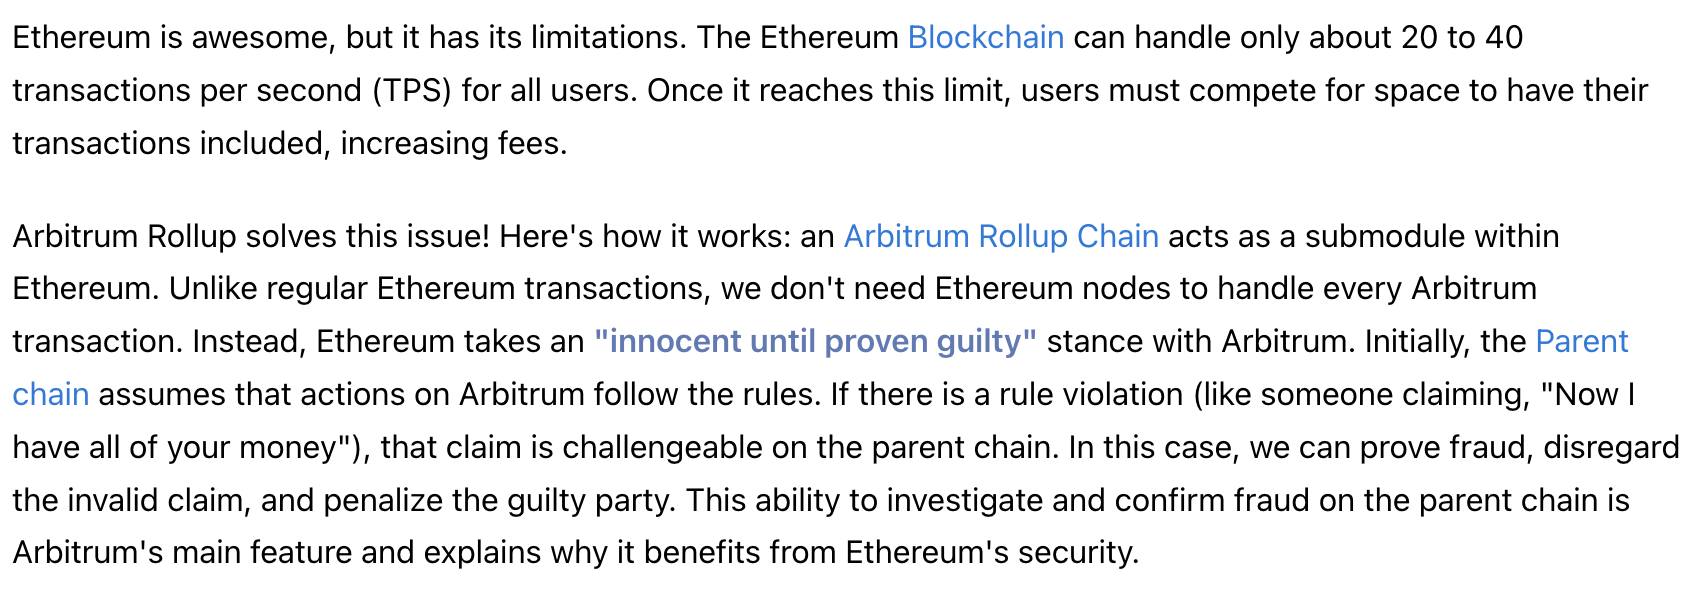
\includegraphics[width = \textwidth]{Arbitrum.png}
    \end{center}
\end{frame}

\begin{frame}{Analogy to Paper Checks}

Has anyone ever paid with a paper check at the grocery store? \\ \pause 

This used to be common! \\ 

Your check would be assumed good until proven otherwise. \\ \pause 

Knowingly writing bad checks is a \textbf{felony}! \\ \pause 

\vfill 

Arbitrum works similarly: you are given the benefit of the doubt, but punished severely for betraying the trust offered you by the system. 
    
\end{frame}


\begin{frame}{Welcome! Today is Wednesday, October 1st!}

\begin{center}
    Office Hours this week will be by appointment over Zoom. \\ 
    Contrary to what I said verbally on Monday, the Midterm is in fact \textbf{October 15}, not Oct 13. 
\end{center}
    
\end{frame}

\begin{frame}{Mango Markets vs. FTX}

\textbf{Q:} Why did Mango Markets fail? \pause \\ 
\textbf{A:} Avraham Eisenberg manipulated the perceived price of his collateral in order to take out and default on large loans. \pause \\ 
\textbf{Q:} Why did FTX fail? \pause \\ 
\textbf{A:} FTX used its customers' funds in a totally different way than they claimed. They were able to hide it because FTX did \ul{not} use transparent smart contracts. 
    
\end{frame}


\begin{frame}{Weakness of DeFi: Miner Extractable Value}

To have your (valid) transaction accepted onto the chain, you must bribe a miner (/staker) to include it in their block. 

    \begin{center}
        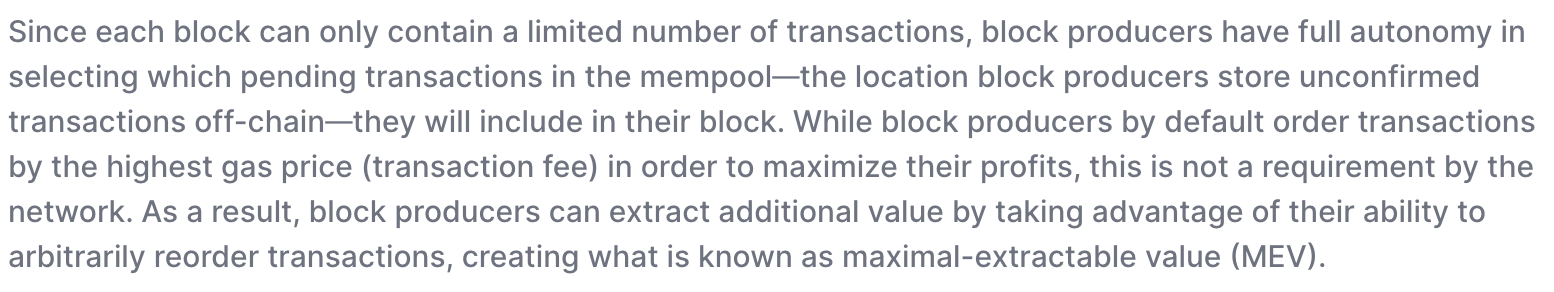
\includegraphics[width = \textwidth]{MEV.png}
    \end{center}

Transactions can be ``sniped''! If I see you submit a transaction and know it's guaranteed to net \$1, I can bribe miners up to \$1 to copy your trade and execute it before you! 
    
\end{frame}

\begin{frame}
\frametitle{Miner Extractable Value and Slippage}

The Blockchain is a highly adversarial environment. 

\bi
\m See Dan Robinson, Georgios Konstantopoulos, \href{https://www.paradigm.xyz/2020/08/ethereum-is-a-dark-forest}{Ethereum is a ``Dark Forest''}
\m See \href{https://arxiv.org/abs/1904.05234}{Flash Boys 2.0}
\m Transaction ordering matters! Miners have power over this
\m \href{https://docs.flashbots.net/}{Flashbots} quite dominant player in this space protocol-wise
\m Many very profitable ``MEV funds'', like crypto HFTs. 
\m MEV tracks demand for \textbf{immediacy} \pause 
\m It is called \textbf{slippage} when your order is filled at a worse price than what was quoted 
\ei

\vspace{2ex}
See \href{https://twitter.com/AnthonyLeeZhang/status/1579181323637641217}{here}

\end{frame}

\begin{frame}{Avoiding Slippage}

To avoid front-runners and slippage, you can 
\bi 
\m Use a protocol that supports setting a \emph{slippage tolerance}: your order is canceled if the price change exceeds your tolerance setting 
\m Paying a higher gas fee to prioritize your transaction 
\m Route your orders through an alternative L2 that polices front-runners
\m Use a protocol like \href{https://docs.arbitrum.io/how-arbitrum-works/timeboost/gentle-introduction}{Arbitrum TimeBoost}
\ei 
    
\end{frame}


\section{Lending Protocols}

\begin{frame}
\frametitle{Collateralized lending}

Collateralized lending in tradfi:
\bi
\m Houses $\implies$ mortgages
\m Cars $\implies$ auto loans
\m Stocks $\implies$ margin loans
\m Firms $\implies$ equipment, real estate, etc. collateralized loans
\m Bonds $\implies$ repo loans
\ei

\end{frame}

\begin{frame}
\frametitle{Collateralized Debt in Tradfi}

\bi
\m I want to buy a house for \$400k, but don't have all the \$\$
\m I tell a bank: ``lend me \$200k; I'll pay you back \$250k; if I don't, you get the house''
\m Key is, the bank only needs to believe that the house is worth over \$250k
\m Collateral provides safety to lenders, making them willing to lend me more \pause
\m IRL, what happens if house price falls below \$300k?
\bi
\m Safe collateral (e.g. U.S. treasuries) doesn't face this risk! 
\m No design is \emph{necessarily} better or worse: someone has to hold the risk, just a question of who is best suited to bear it 
\ei
\ei

\end{frame}

\begin{frame}{Margin Calls}

\begin{center}
    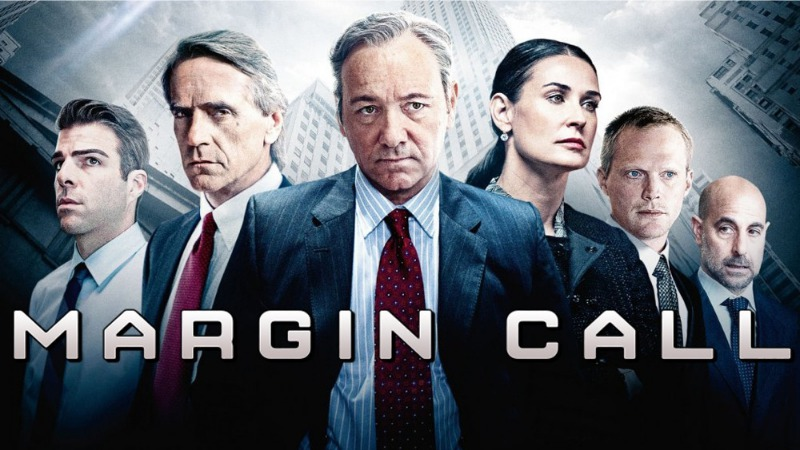
\includegraphics[width = \textwidth]{Margin-Call.jpg}
\end{center}
\bi 
\m A much better finance movie than The Big Short 
\ei 
\end{frame}

\begin{frame}{Margin Call: Example}

\bi 
\m I put in \$10,000 to buy \$20,000 of stock with a \textbf{maintenance margin} of 30\%\footnote{FINRA minimum is 25\%}. The \textbf{margin} is (my equity / the total position), so 50\% initially. I am in compliance because 50\% exceeds 30\%. 
\bi 
\m The broker lends me the other \$10,000 \pause 
\ei 
\m The value of the stock drops to \$14,000  
\m My \ul{equity} is now \$14,000 - \$10,000 = \$4,000 
\m My \ul{margin} is now \$4,000/\$14,000 = 28\% \pause 
\m My broker makes a \textbf{margin call}: I need to deposit \$200 to bring my \ul{margin} back up to the required 30\% \pause 
\m This happens because the \ul{collateral} is the stock itself, which has uncertain value 
\m If I refuse to meet the margin call, the broker \ul{liquidates} my position: He sells the stock to make himself whole. He pays me back what's left of my equity, locking in my loss. 
\ei 
    
\end{frame}


\begin{frame}
\frametitle{Defi Collateralized Lending}

\bi
\m Collateralized lending requires:
\be
\m System for collateral custody
\m System for evaluating collateral value and ``margin calls''
\ee
\m Defi good at 1., can have a ``collateral pot'' smart contract
\m Defi less good at 2. (See Mango Markets)!
\ei

\end{frame}

\begin{frame}
\frametitle{Aave (Finnish for ``Ghost'')}

\bi
\m Deposit \$150 of ETH into Aave
\m Aave allows you to borrow up to $\$150\times (1-\textrm{margin})$ of other tokens\pause
\bi
\m Where do other tokens come from?
\m Others are lending into Aave to borrow other tokens
\ei \pause
%\m All loans are \ul{overcollateralized}: collateral worth more than borrowing \pause
\m If ETH price falls, so collateral worth \$100, if loans more than $\$100\times \gamma$, borrower choices:
\bi
\m Add more collateral (``margin call'')
\m Reduce leverage (pay back loans)
\m Liquidate collateral 
\ei \pause
\m With a sufficiently strict smart contract that can liquidate quickly, this protocol should never lose money
\ei

\end{frame}

\begin{frame}
\frametitle{Aave Rates}
Lenders in Aave play the role of ``brokers'', earning yield:
\begin{center}
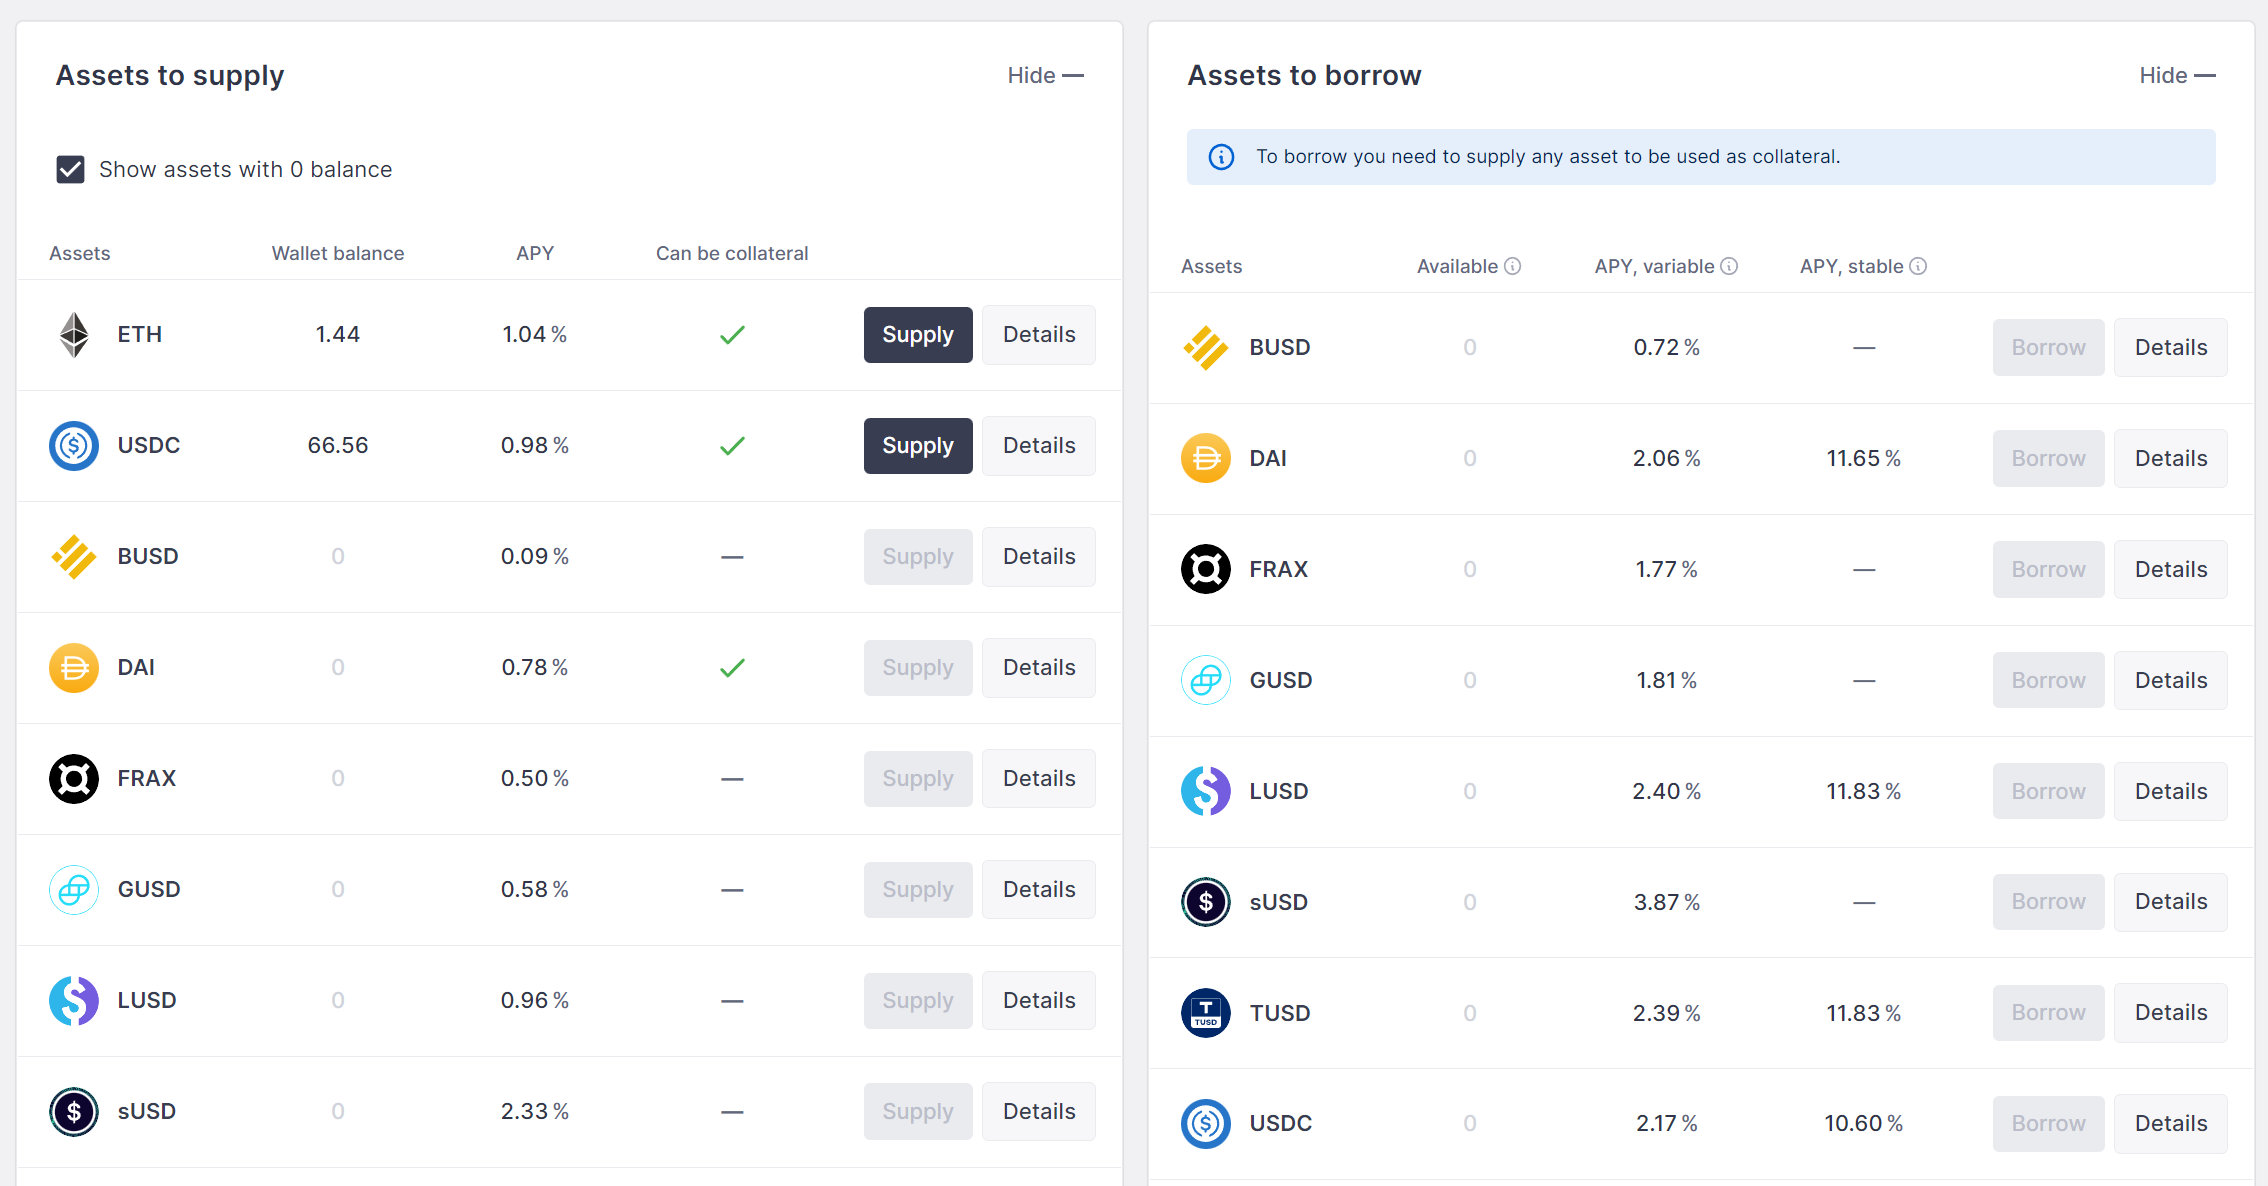
\includegraphics[width = 0.9\textwidth]{pics/aave_rates.png}
\end{center}

\end{frame}

\begin{frame}
\frametitle{Who uses Aave?}

Why would you lend to Aave?
\bi
\m Have many tokens but few opportunities, want returns
%\m Have tokens, want to borrow
\ei \pause
Why would you borrow from Aave?
\bi
\m Have few tokens but many opportunities, want \ul{leverage}
\bi \pause
\m Leverage: hold \$100 of assets with only \$50 of cash
\m Mortgages, margin buying\ldots
%\m Borrow stablecoins against ETH
\ei \pause
%\m Want to short tokens
\m Need tokens for some utility function
\bi
\m Borrow tokens to vote on governance proposals?
\ei
\ei

\end{frame}


\begin{frame}
\frametitle{Rate Setting on Aave}

\bi
\m Aave interest rates based on \ul{utilization}: 
\[
U=\frac{Total\ Borrowed}{Total\ Lent}
\]
\m Interest rate is higher when $U$ is higher
\m When lots of people want to borrow, what happens? \pause
\bi
\m $U$ increases, decreasing borrowing, increasing lending
\m Pool equilibrates at a larger size, possibly higher rate
\ei \pause
\m When few people want to borrow, what happens? \pause
\bi
\m $U$ decreases, decreasing lending, increasing borrowing
\m Pool equilibrates at a smaller size
\ei \pause
\m When some lenders need to withdraw, what happens?
\bi
\m $U$ increases, so remaining lenders have incentive to stay in pool
\m New lenders higher incentive to join pool
\m Borrowers have incentives to scale down
\ei
\ei

\vspace{2ex}
\footnotesize

See \href{https://docs.aave.com/risk/liquidity-risk/borrow-interest-rate}{Aave website}

\end{frame}


\begin{frame}
\frametitle{The Defi Fixed Income Ecosystem}

Borrowing/lending protocols imply there is now an ecosystem of fixed income strategies available in defi:
\bi
\m Pure borrow/lend (\href{https://aave.com/}{Aave}, \href{https://compound.finance/}{Compound})
\m Stablecoin market making (\href{https://curve.fi/}{Curve}, \href{https://www.convexfinance.com/}{Convex})
\m Clones/variants on other chains besides ETH
\m Frontiers: uncollateralized lending, fixed rates\ldots
\ei

\end{frame}


\begin{frame}{Fractional Reserve Banking with Infinifi}

\vfill 
\begin{center}
    \href{https://infinifi.xyz/}{infinifi.xyz}
\end{center}
\vfill 
    
\end{frame}

\begin{frame}{Fractional Reserve Banking with Infinifi}

Fractional reserve banking/ Maturity transformation in DeFi 

\begin{center}
    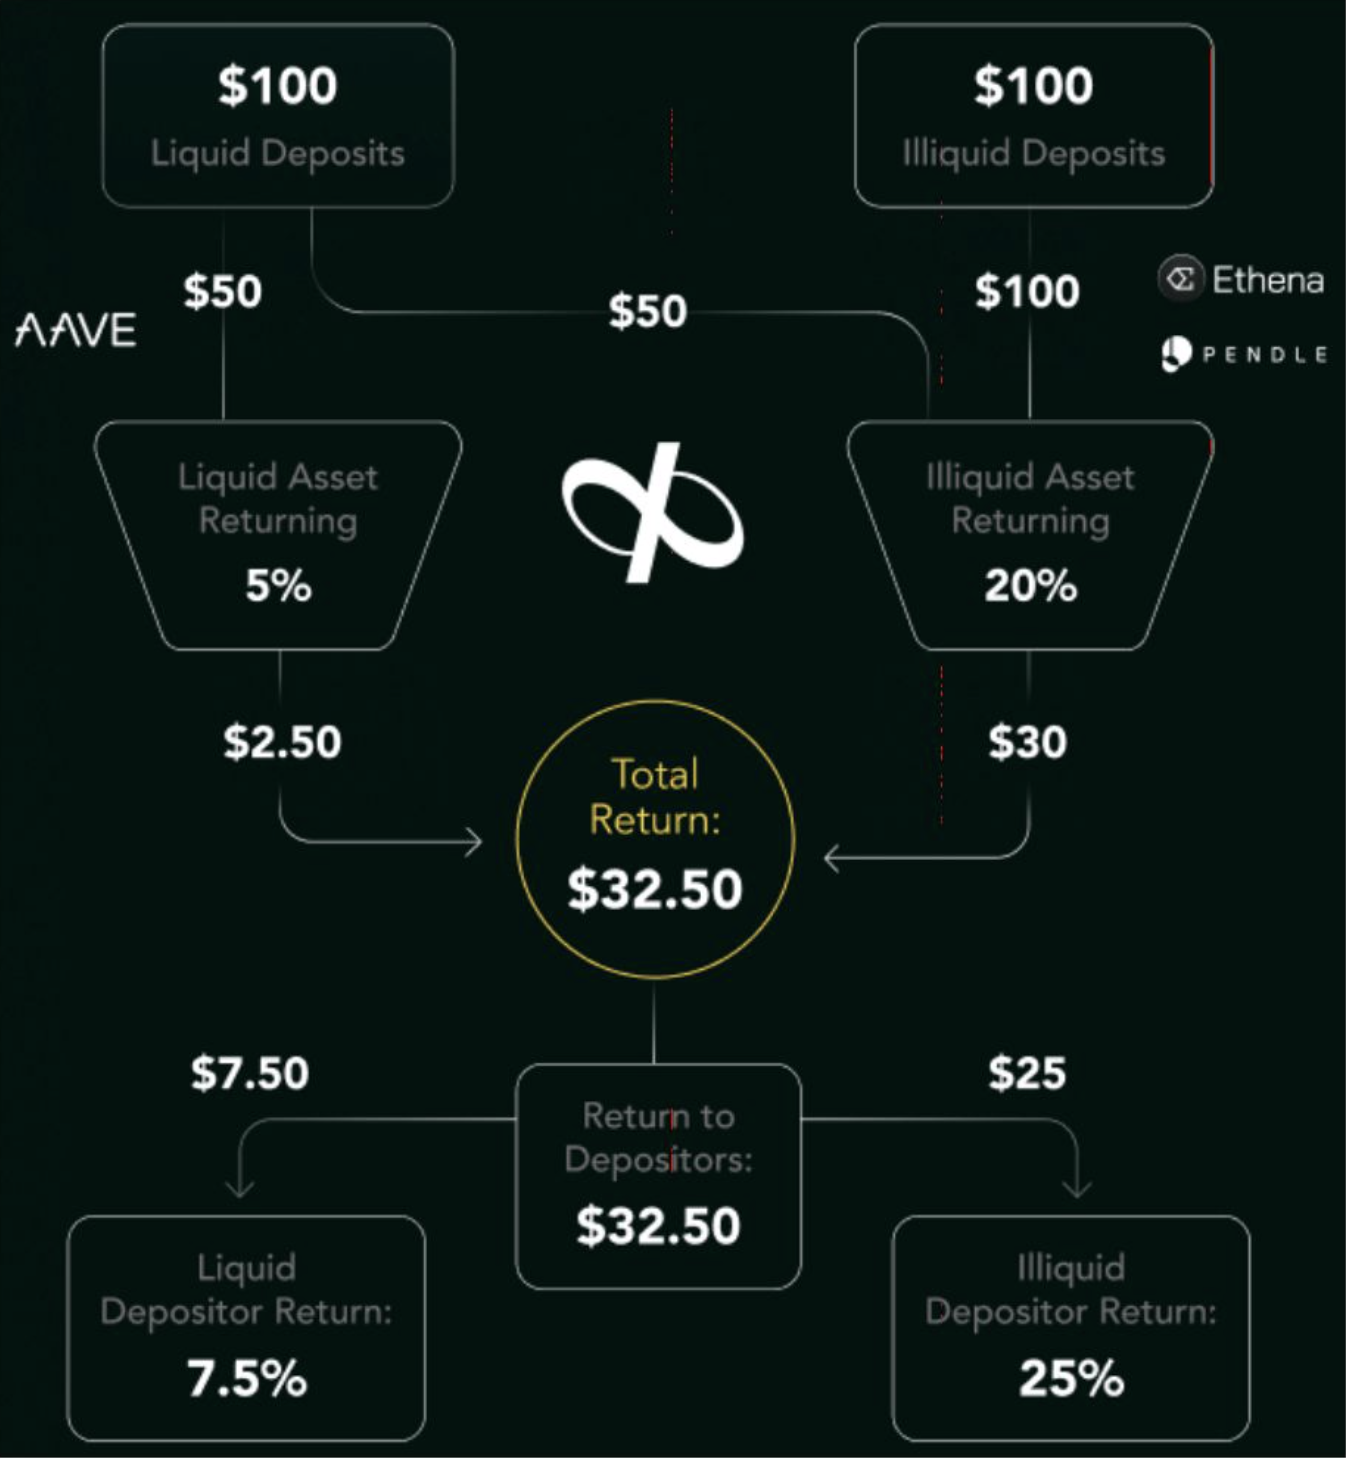
\includegraphics[height = 0.6\textheight]{infinifi.png}
\end{center}

Will this work without deposit insurance? \pause 
\bi 
\m My prediction: This protocol is vulnerable to bank runs. 
\ei 
    
\end{frame}


\begin{frame}{Uncollateralized lending relies on \ul{Reputation}}

\vfill
\begin{center}
    \href{https://www.ledgerscore.com/}{ledgerscore}
\end{center}
\vfill
    
\end{frame}


\begin{frame}
\frametitle{Web3 Identity}

\bi
\m What's in a physical wallet? \pause 
\bi
\m Cash, credit cards, and \ul{identity cards}!
\ei
\m An ID card is an item which: 
\bi
\m Proves who you are (student, gym member\ldots) 
\m Gives you certain rights (discounted tickets, gym access\ldots)
\ei
\m ID cards are not transferrable!
\m We can create web3 ID cards through \ul{non-transferable tokens}
\m May 2022 \href{https://papers.ssrn.com/sol3/papers.cfm?abstract_id=4105763}{Weyl-Ohlhaver-Buterin} paper: \ul{soulbound tokens} as the basis of web3 identity
\ei

\end{frame}

\begin{frame}
\frametitle{Project Ideas: SBTs and Web3 Identity}

Identity very young, essentially no apps yet, so a good area for class projects! Many taken from \href{https://papers.ssrn.com/sol3/papers.cfm?abstract_id=4105763}{WOB paper}
\bi
\m What are good SBT use cases?
\bi
\m Diplomas? Employment history?
\m ``Social credit scoring''? Rewards for good deeds?
\m Some examples: \href{https://twitter.com/otterspace_xyz}{Otterspace}, \href{https://twitter.com/discoxyz}{Disco.xyz}, \href{https://lens.xyz/}{Lens}, and \href{https://twitter.com/AnthonyLeeZhang/status/1577104530348859392}{others}
\ei
\m How should SBTs work?
\bi
\m Who gets to bestow SBTs?
\m Who gets to remove SBTs? Privacy? ``Scarlet letter'' SBTs?
\m How do we solve ``walking away from my soul''?
\ei
\m In a world where SBTs are ubiquitous, what functions are enabled that can't exist yet?
\bi
\m SBT-based uncollateralized lending? 
\m SBT-ML and recommendation filtering?
\m SBT-gated social organization? Private clubs? Dating apps?
\ei
\m More broadly, what are some implications of ``native composability'' that the world hasn't realized yet?
\ei

\end{frame}


\begin{frame}
\frametitle{Native Composability}

\bi
\m Web3 (DeFi) gives us \ul{native composability}
\m In web2, app functions and data are \ul{closed by default}
\bi
\m Facebook, Google, Twitter have internal functions, data\ldots
\m But can't access each other's data + functions, unless they specifically build APIs to do so
\m If Google doesn't want your app to ``plug into'' Google maps, hard for you to do so
\ei \pause
\m In web3, app functions + data are \ul{open by default}!
\bi
\m Very hard for Uniswap to ``stop'' your app from calling Uniswap functions!
\m All data is on chain: everyone can see every app's data!
%\m Will be important for ``vampire attacks'' in tokenomics lecture in a few weeks
\ei \pause
\m Harder to construct ``walled garden ecosystems'', lower barriers to entry + less incumbent advantage
\ei

\vspace{2ex}
\small
See ``Appendix: Composability'' in Saffron Huang's post \href{https://saffron.mirror.xyz/MEz-IkBGe36LdLn2VVA6grv9FWxU2NdQpVubF6T1ZJE}{here}

\end{frame}

\begin{frame}{Faster Horses?}
\centering
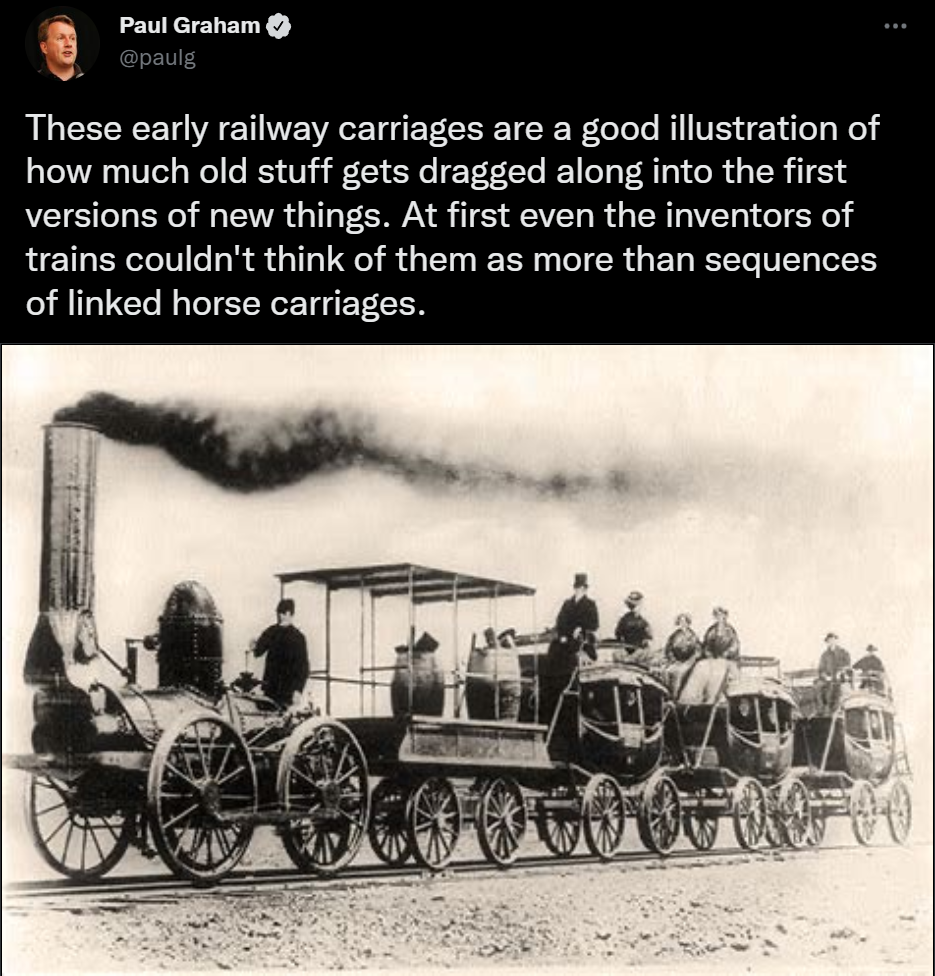
\includegraphics[width=0.7\textwidth]{pics/paulgrahamtweet.png}

\end{frame}

\begin{frame}
\frametitle{Interest Rates in Traditional Finance}

\begin{center}
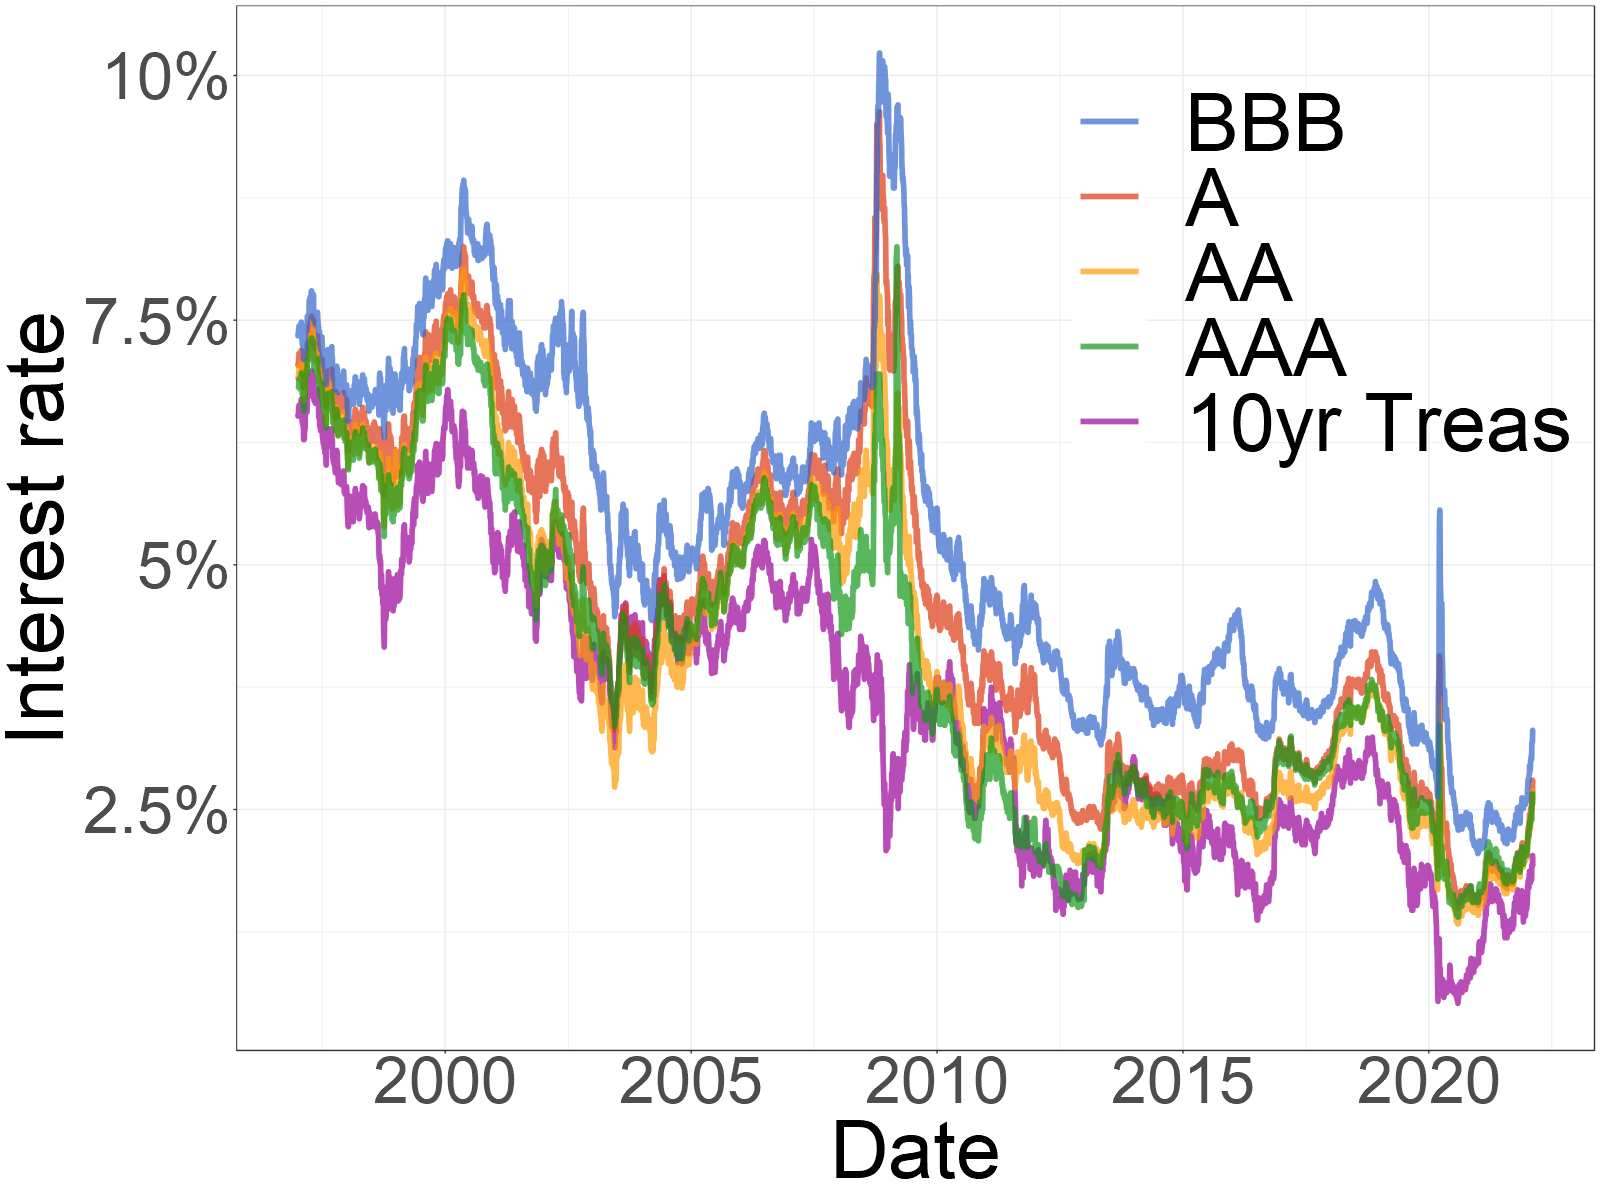
\includegraphics[width=.9\textwidth]{pics/bonds.png}
\end{center}

\end{frame}

\begin{frame}
\frametitle{Interest Rates in Defi}

\begin{center}
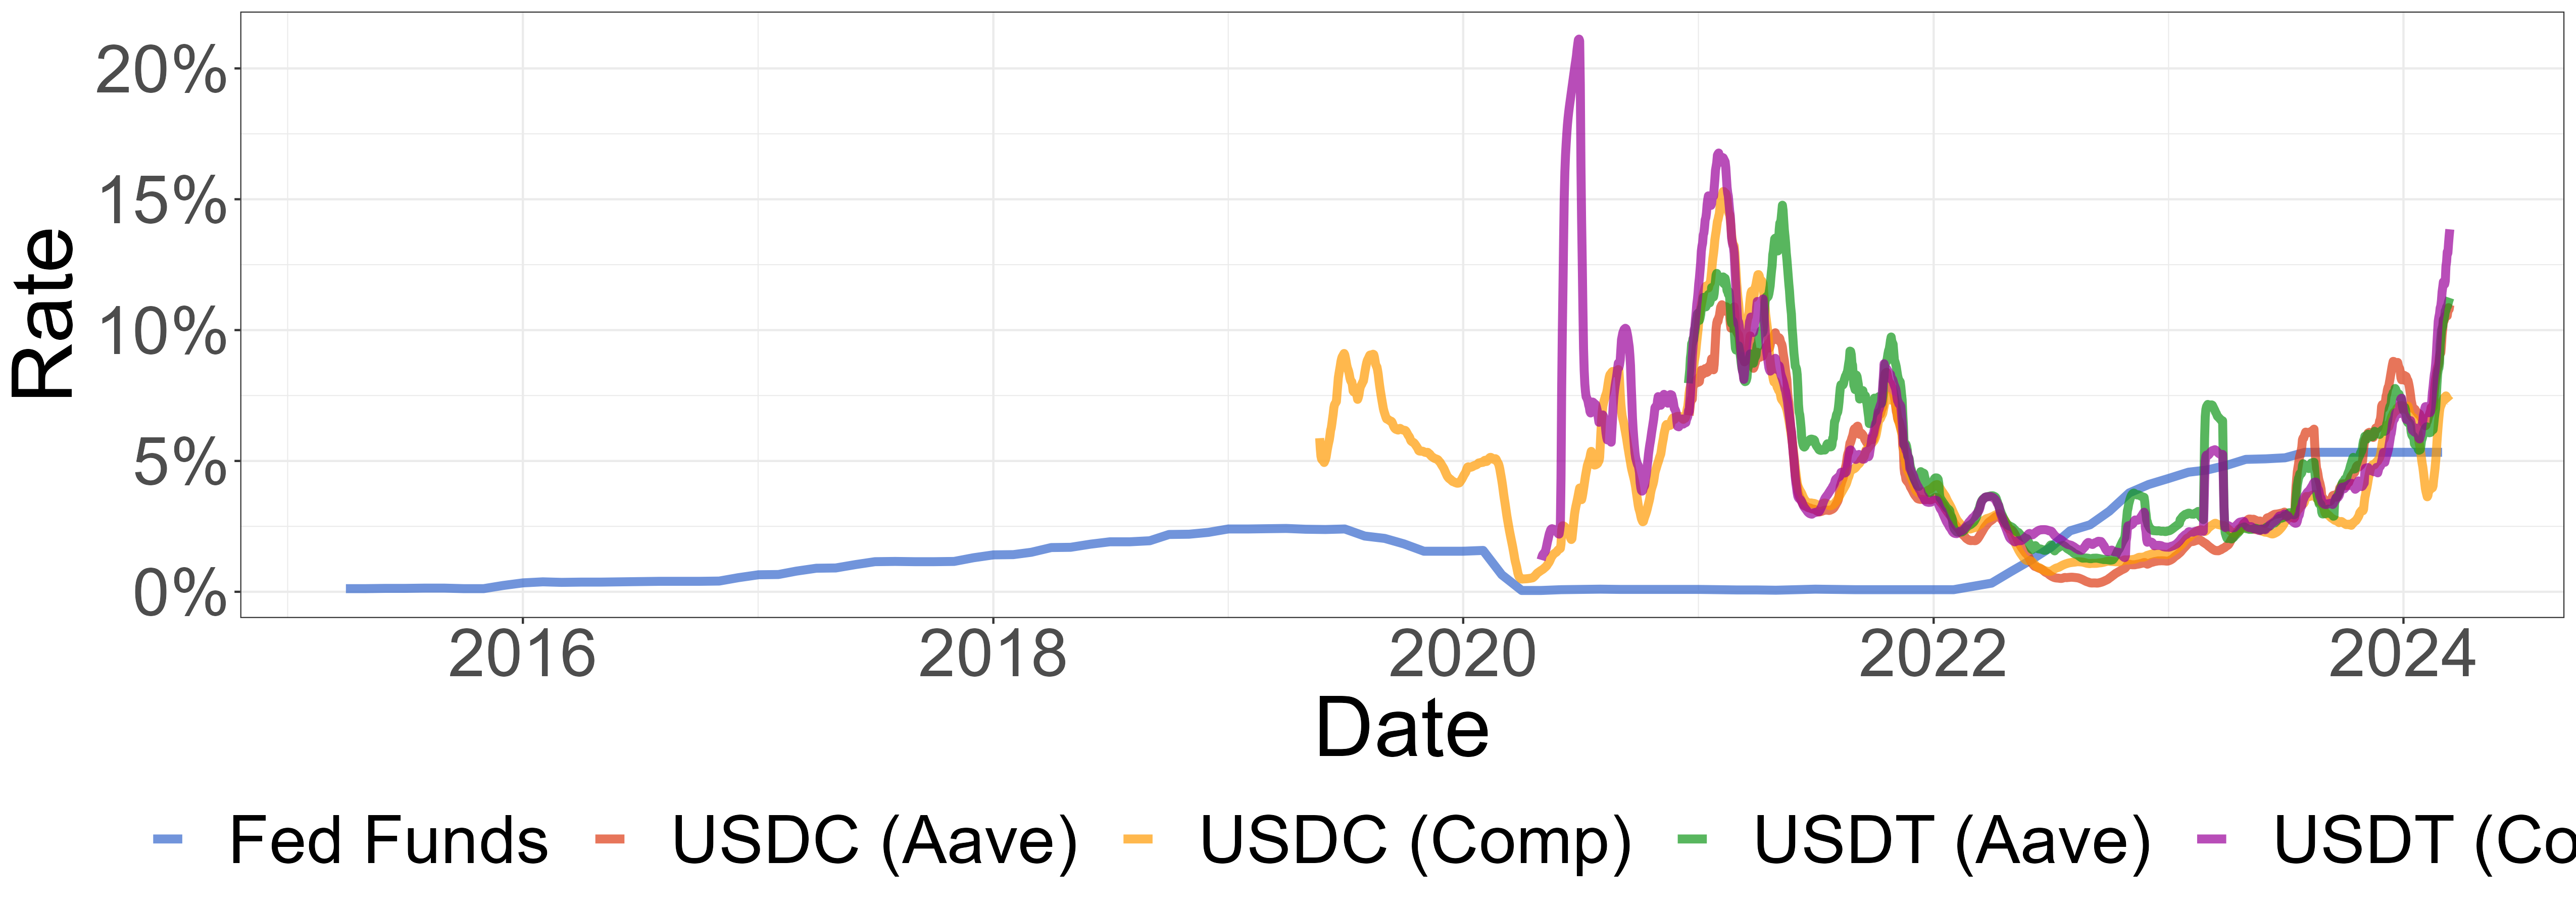
\includegraphics[width=\textwidth]{ratesplot.png}
\end{center} 


\end{frame}

\begin{frame}
\frametitle{Liquidation}

I borrow \$400k against my \$500k house
\bi
\m Ideal case: I pay back \$400k, live in my house
\m Non-ideal: I can't make payments, bank sells my house and keeps \$400k
\m Safety of bank's mortgage debt depends on how well they can ``liquidate collateral''
\m How does a smart contract play the role of the bank in liquidating collateral?
\ei

\end{frame}

\begin{frame}
\frametitle{Ideal Liquidation}

\bi
\m Suppose you borrow \$100 USD against \$150 of ETH
\m ETH price drops to be worth \$149, so your position must be liquidated
\m ``Ideal'' procedure:
\bi
\m Protocol detects that ETH price dropped, your position is insolvent
\m Protocol sells ETH to pay down your debt
\ei
\m Is this possible? \pause
\m Requires: 
\bi 
\m An Oracle to tell it relevant prices 
\m Either a human in the loop or a replenishing supply of gas to continually check prices and liquidate as necessary  
\m Someone to whom to sell the ETH  
\ei 

\ei

\end{frame}


\begin{frame}
\frametitle{Liquidation in Practice: Sale Mechanism}

\bi
\m Sell to AMM?
\bi
\m Large order, may move prices too much
\ei
\m Sell to humans? How? \pause
\m \textbf{Aave/Compound:} fixed price, below current oracle price, see \href{https://docs.aave.com/risk/v/master/asset-risk/risk-parameters}{risk parameters} \pause
\bi
\m Fast, safe, but potentially leaves a lot of money on the table 
\ei \pause
\m \textbf{Maker}: collateral sold in descending auction
\bi
\m Slower, but very likely to get more money 
\ei
\ei

\end{frame}

\begin{frame}
\frametitle{Risks: Oracle Risk}

\bi
\m Unlike AMMs, collateralized lending systems require \ul{oracle inputs} for prices
\m Risk factor: if oracle gets manipulated, lending system is at risk!
\m How would you attack Aave through oracle manipulation? \pause
\be
\m Deposit \$100 Xtoken as collateral
\m Manipulate oracle, make Aave think \$100 Xtoken is worth \$100,000
\m Borrow \$50,000 USDC against your Xtoken
\m Default: you've just traded \$100 Xtoken for \$50,000 USDC!
\ee
\m See \href{https://medium.com/beaver-smartcontract-security/defi-security-lecture-7-price-oracle-manipulation-d716cdeaaf77}{here} for other examples of oracle attacks
\m \ul{Chainlink} is the main oracle provider
\bi
\m Uses off-chain data! Ironic, as it's more ``principled'' to use on-chain data
\ei
\ei

\end{frame}


\begin{frame}
\frametitle{Alleviating Oracle Risks?}

\begin{center}
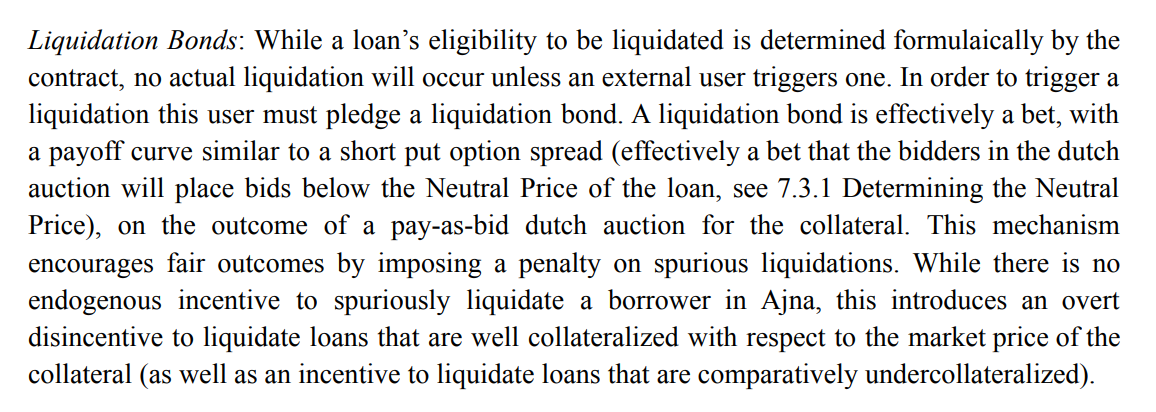
\includegraphics[width=\textwidth]{pics/ajna.png}
\end{center}

\smallskip
\footnotesize

Source: \href{https://www.ajna.finance/pdf/Ajna_Protocol_Whitepaper_01-11-2024.pdf}{Ajna protocol} \newline \pause 

Put simply: Ajna makes loans that fail margin \emph{eligible} for liquidation. A human must always ``pull the trigger'', and that human is penalized \emph{ex-post} if the collateral turns out to be good after all (a ``\textbf{spurious liquidation}''). 

\end{frame}


\begin{frame}{Welcome! Today is Wednesday, October 8}

\begin{center}
    Homework 3 is due Monday. Some students have observed that Uniswap defaults to a high gas fee -- this can be changed in the transaction settings.\\ \vfill 

    Also for Monday: read ``In Praise of Ponzis'' by Dror Poleg: \\ 
    \href{https://www.drorpoleg.com/in-praise-of-ponzis/}{https://www.drorpoleg.com/in-praise-of-ponzis/} \\ \vfill 

    The second and final \textbf{Midterm Exam} is \textbf{Wednesday, October 15}. The Practice Midterm is on Canvas. The practice answer key will be revealed on Friday. 
    
\end{center}
    
\end{frame}

\begin{frame}{In the News: Key Cybersecurity Law Expires}

\begin{center}
    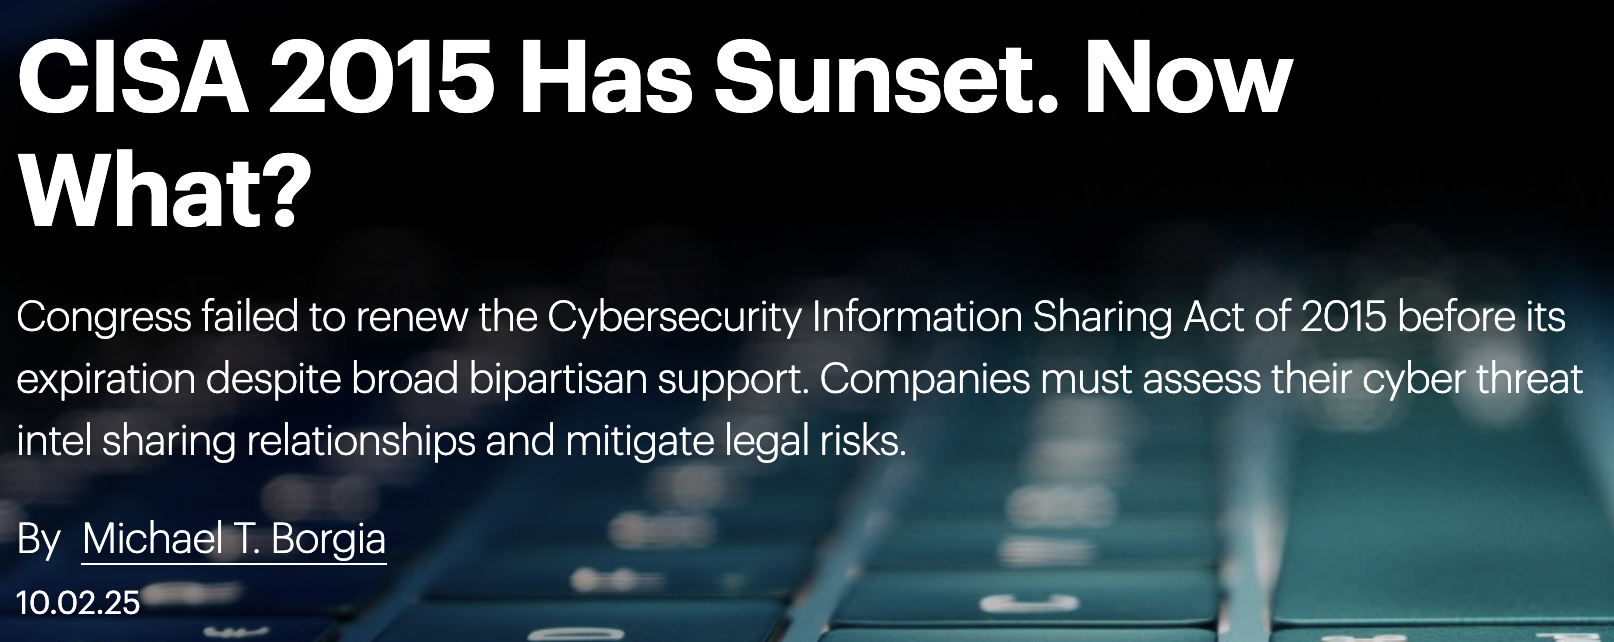
\includegraphics[width = \textwidth]{cisa.png}
\end{center}
    
\end{frame}

\begin{frame}{What does this mean?}

\begin{itemize}
    \item A patchwork of federal and state laws restrict companies' ability to share data. Two main concerns: 
    \begin{itemize}
        \item \textbf{Privacy}: companies may compromise the privacy of their users by sharing data 
        \item \textbf{Antitrust}: companies who share data may be accused of colluding to raise prices instead of competing in the free market 
    \end{itemize}
    \item From 2015 to 2025, companies had \textbf{safe harbor} to share data concerning cybersecurity threats with each other and the federal government 
    \item With this protection gone, companies may stop sharing information with each other. 
\end{itemize}
    
\end{frame}


\begin{frame}{In the News: Arc White Paper}

\begin{center}
    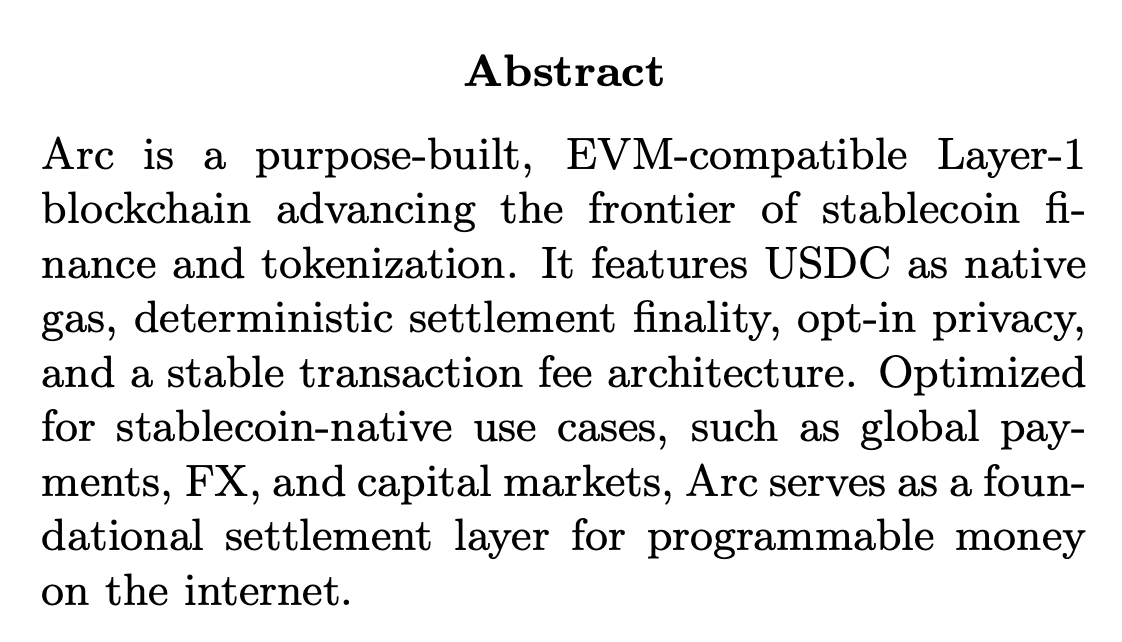
\includegraphics[width = .9\textwidth]{arc_abstract.png}
\end{center}

\begin{itemize}
    \item \textbf{Circle}, the issuer of USDC (\#2 largest stablecoin), encourages developers to ditch Ethereum for Arc 
\end{itemize}
    
\end{frame}


\begin{frame}{In the News: Arc White Paper}

Why denominate gas fees in USDC (Circle's USD stablecoin)? \\ 
My inbox yesterday: 

\begin{center}
    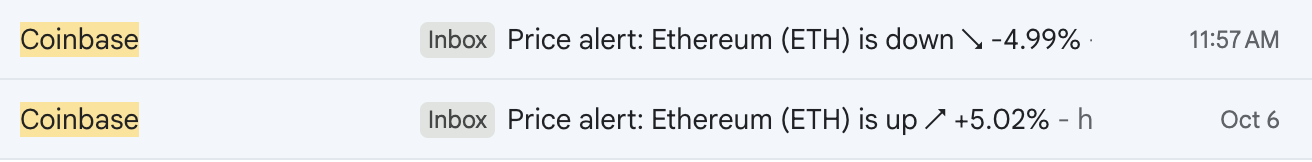
\includegraphics[width = \textwidth]{ethereum_price.png}
\end{center} 

\end{frame}

\begin{frame}{In the News: Arc White Paper}

\textbf{Circle's Philosophy}: ``It is built on the conviction that the future of finance and commerce is not a wholesale replacement of the old, but a synthesis of the new and the established: the programmability of smart contracts with the enforceability of law (i.e., GENIUS Act); the efficiency of blockchain with the stability of fiat-backed currency; and the transparency of public ledgers with the privacy required for commercial transactions.'' 
    
\end{frame}

\begin{frame}{In the News: Arc White Paper}

\begin{itemize}

\item ``Arc will rely on a permissioned, \textbf{Proof-of-Authority (PoA)} validator set composed of a limited number of known, established, and geographically distributed institutions held to high standards of accountability and operational guarantees.''

\item The Arc project \textbf{gives up on decentralization} and \textbf{gives up on value appreciation} in order maximize its utility and stability for the current, existing financial system. 

\m Giving up on value appreciation is a big deal! Early adopters cannot capture the value of the future adoption that they encourage. 
\end{itemize}
    
\end{frame}


%\begin{frame}
%\frametitle{Risks: Operational Risk}

%\bi
%\m Lending code particularly tricky to get right, because your funds are locked in contract, and can be lent out
%\m How does this differ from AMM trading? \pause
%\m Many examples, such as \href{https://rekt.news/cream-rekt/}{CREAM finance}, \href{https://www.cnbc.com/2021/10/03/162-million-up-for-grabs-after-bug-in-defi-protocol-compound-.html}{Compound}
%\ei

%\end{frame}


\begin{frame}
\frametitle{Fire Sale and Contagion: a Vicioius Cycle}

Recall the discussion of \textbf{leverage} (borrowing money) and \textbf{liquidations} (e.g. a margin call). 

\bi
\m Suppose price of ETH drops
\m People borrowing against ETH get liquidated, so ETH gets sold
\bi 
\m This is called a \textbf{fire sale}
\ei 
\m Selling pressure pushes down ETH prices\ldots
\m Leading to more liquidations\ldots 
\bi 
\m This is called \textbf{contagion}
\ei 
\ei

\end{frame}


\begin{frame}
\frametitle{Systemic Fragility}

\begin{center}
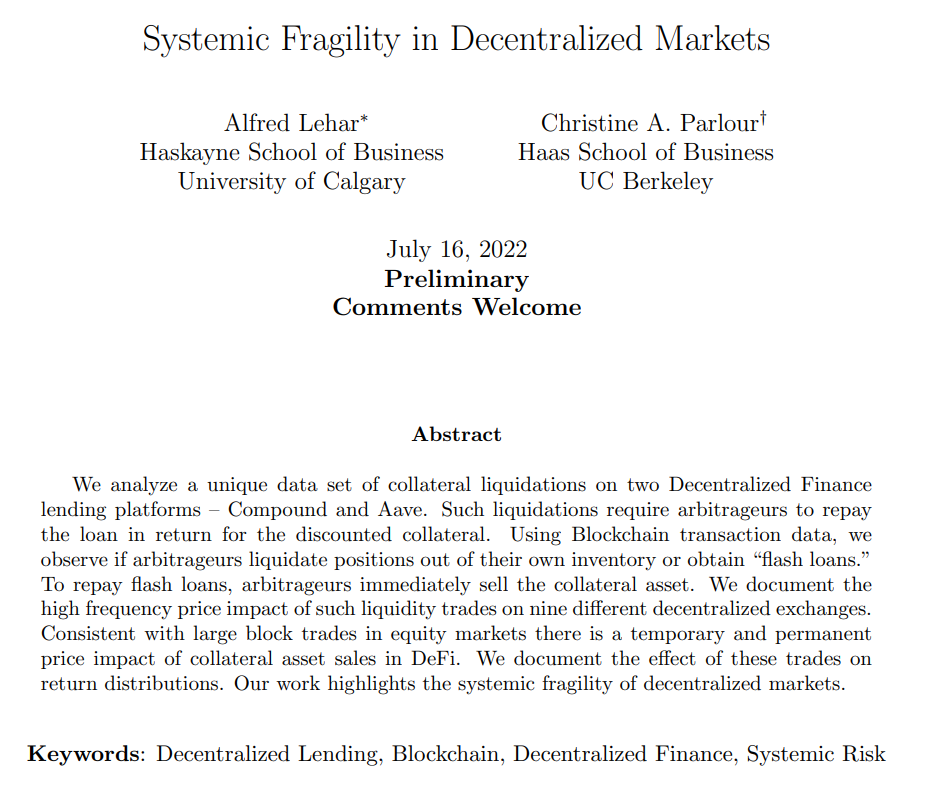
\includegraphics[width=.7\textwidth]{pics/systemicfragility1.png}
\end{center}

\href{https://papers.ssrn.com/sol3/papers.cfm?abstract_id=4164833}{Source}

\end{frame}

\begin{frame}
\frametitle{Flash Loans}

\bi
\m Unlike traditional finance, transactions in defi are \ul{atomic}: either the whole tx finishes, or none of it does
\m Enables a cool trick called \ul{flash loans}
\m You can borrow a very large amount of money, unsecured\ldots
\m {\ldots}as long as you pay it back \emph{in the same transaction!}
\m If you can't pay back the money, tx fails, so you never borrowed it in the first place!
\m Flash loans available from Aave, Compound\ldots
\ei

\end{frame}


\begin{frame}{Triangular Arbitrage in Traditional Currency Markets}

\begin{center}
    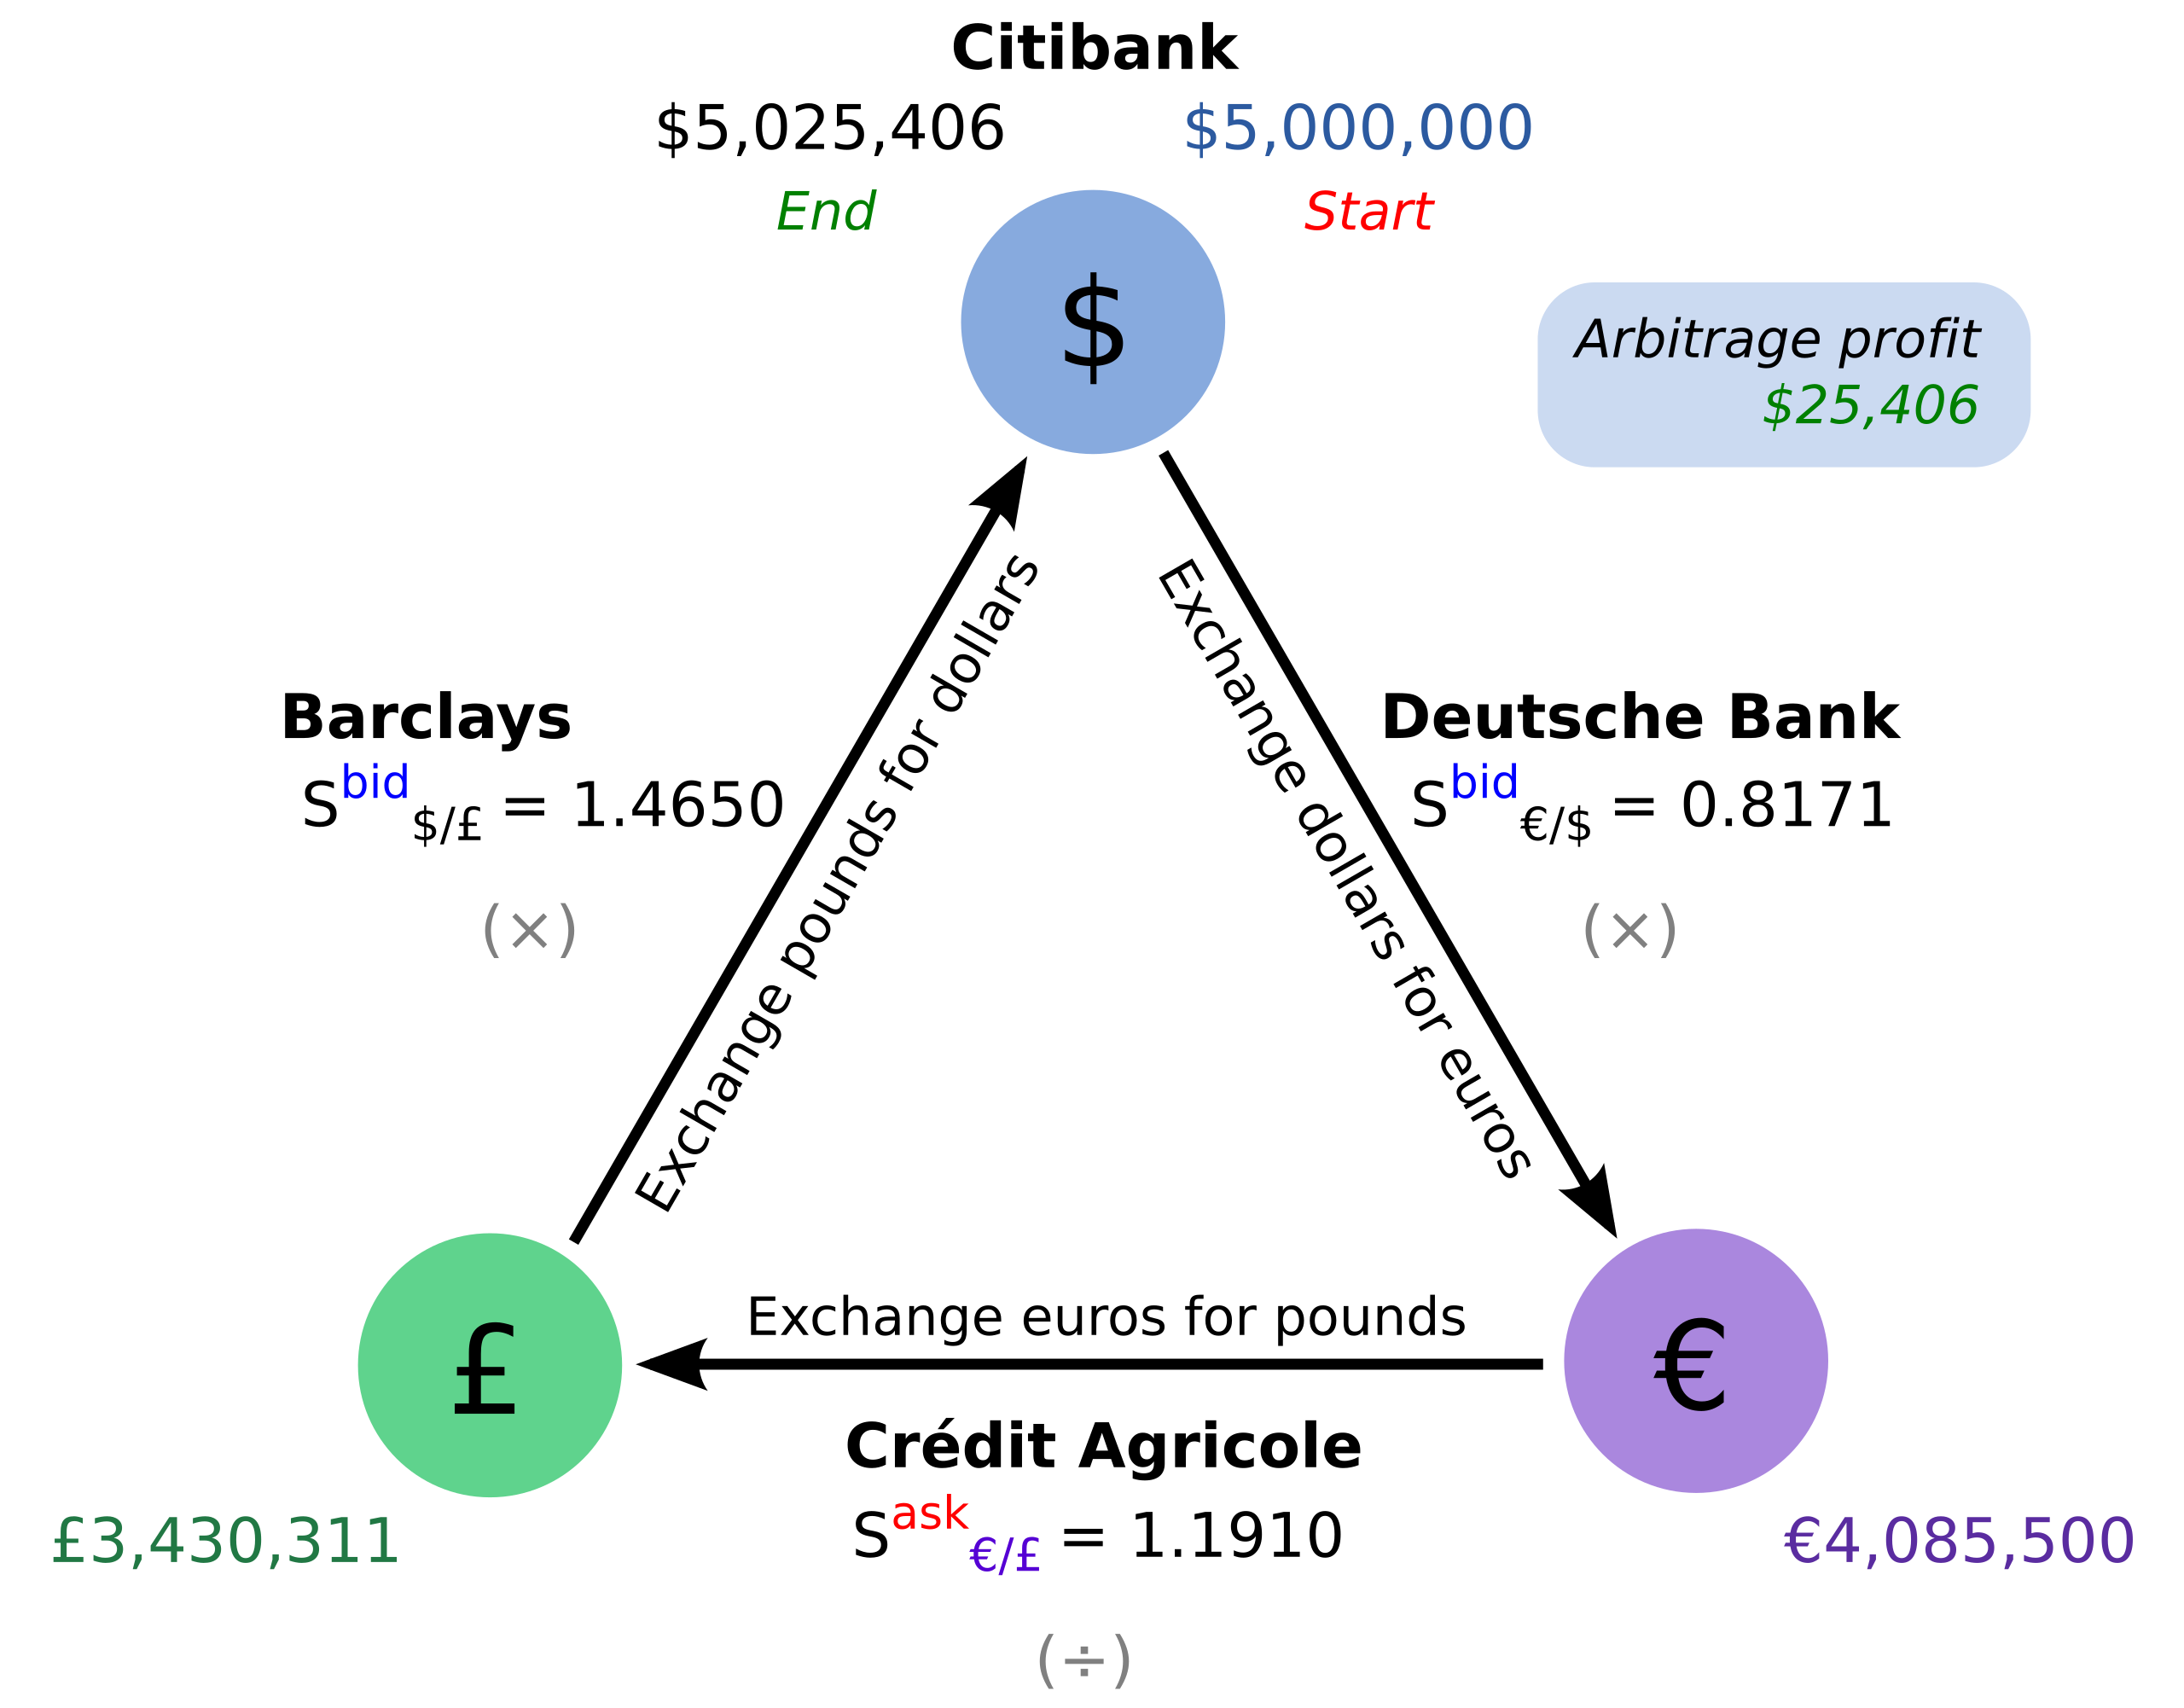
\includegraphics[width = .7\textwidth]{triangular_arbitrage.png}
\end{center}

The elimination of triangular arbitrage imposes strict limits on bilateral exchange rates \textbf{in frictionless markets}: if Euros are X/dollar, and Pounds are Y/dollar, Euros \ul{must} be (X/Y)/Pound. 
    
\end{frame}

\begin{frame}
\frametitle{Flash Loans: Consequences}

\bi
\m In tradfi, \ul{arbitrage} requires \ul{capital} and \ul{infrastructure}
\bi
\m Hedge funds can do trades you can't 
\ei
\m In DeFi, infrastructure accessible by default; flash loans democratize capital
\m If there are arbitrage opportunities, anyone can extract them!
\bi 
\m \ul{``Triangular arbitrage''} becomes close to frictionless! 
\ei 
\ei

\end{frame}

\begin{frame}
\frametitle{Case Study: The Cream Finance Hack}

\bi
\m Zhang writes about the \href{https://medium.com/@anthonyleezhang/how-cream-finance-lost-130-million-in-one-trade-1853c83c20b3}{CREAM finance attack}
\m Attacker submitted a \href{https://etherscan.io/tx/0x0fe2542079644e107cbf13690eb9c2c65963ccb79089ff96bfaf8dced2331c92}{bundle of 20 transactions}, borrowed a billion dollars, made \$130mil, paid \$6,500 in gas fees!
\m Details complicated, but essentially:
\bi
\m CREAM finance allows you to borrow collateralized, borrowing amount determined by price oracle
\m Attacker builds a large collateral + debt position through ``rehypothecation''
\m Flash borrow \$1.5bil, deposit in CREAM
\m Manipulate price, to make CREAM think \$1.5bil of collateral is worth \$3bil
\m Borrow \$2bil of ETH against collateral, worth only \$1.5bil
\m Default on collateral, keep \$2bil in ETH, pay back \$1.5bil flash loan, keep \$500mil ish in profit (actually only \$130mil)
\ei
\ei

\end{frame}

\begin{frame}
\frametitle{Case Study: The Beanstalk Attack}

\bi
\m \href{https://twitter.com/AnthonyLeeZhang/status/1515702276396130307}{Tweet thread} on the Beanstalk attack 
\m Beanstalk is an algo-stablecoin, holds collateral 
\bi 
\m A \textbf{stablecoin} is a coin intended to trade always at \$1
\m An \textbf{algo-stablecoin} tries to do this without relying on the regulated banking system (recall ``Terra'') 
\ei 
\m Governance done through equity tokens: majority token vote approves any change \pause 
\m \textbf{Does this sound like a good idea?} \pause 
\m Attacker proposed: ``send entire treasury to my address'' \pause 
\m Flash borrowed a bunch of equity tokens, passed the proposal, took all the money!
\ei

\end{frame}

\begin{frame}
\frametitle{Flash Loans: Consequences}

Consequences of flash loans:
\bi
\m ``On-chain'' price oracles (for collateral valuation, derivatives settlement, etc.) very rarely used: often attackable
\m Hacky solution: just use Binance prices, imported through Chainlink, instead
\bi 
\m Binance is a ``traditional exchange'' that holds on-chain assets for you 
\m These have a ``human in the loop'' 
\ei 
\m Governance attacks rarer: beanstalk a unique case
\m The threat of ``51\% attacks'' is why most modern protocols do not operate on unconstrained democracy. 
%\bi
%\m However, Curve/Convex demonstrates that the ``market for votes'' -- flash loans aside -- still very important
%\ei
\ei

\end{frame}



\section{Derivatives}


\begin{frame}{Derivatives}

\textbf{Derivatives} are simply contracts that take the prices of other contracts (or commodities) as inputs. Popular derivatives include: 

\bi 
\m Synthetics: I pay you the price of an asset $X$ 
\bi 
\m Exposed to counterparty risk! 
\m \textbf{Clearinghouses} are trusted intermediaries who mitigate counterparty risk, e.g. by holding collateral 
\ei 
\m Options: I pay you (the greater of 0 or) the price of a stock $x$ minus the strike price $k$ at the expiration date $t$ (this example is called a ``call option''). 
\m Futures: I pay you the price of $X$ at date $t$
\m $X$ could be a price, an interest rate, a ratio of prices, let your imagination go wild... 
\ei 
    
\end{frame}

\begin{frame}
\frametitle{Options}

\bi
\m Off-chain options on crypto fairly widely available: Binance, Deribit, FTX\ldots
\m Liquidity remains low (high bid-ask spread, volatile prices) 
\m Many projects trying to build on-chain options. A few classes of approaches:
\bi
\m Standard options: \href{https://premia.finance/}{Premia}
\m ``Power perpetuals'', gamma exposure through convex futures: \href{https://squeeth.opyn.co/?ct=US}{Opyn Squeeth}
\m Replicating options through AMM LP positions: \href{https://twitter.com/Panoptic_xyz}{Panoptic}
\ei
\m Application layer:
\bi
\m Structured products: \href{https://www.ribbon.finance/}{Ribbon Finance}, \href{https://friktion.fi/}{Friktion}
\ei
\m Some other projects: \href{https://twitter.com/dopex_io}{dopex}, \href{https://twitter.com/lyrafinance}{Lyra}, \href{https://twitter.com/ryskfinance}{rysk}, \href{https://primitive.xyz/}{Primitive}
\ei

\vspace{2ex}
\href{https://twitter.com/AnthonyLeeZhang/status/1579176369367703553}{Others}

\end{frame}

\begin{frame}
\frametitle{Futures, Synthetic Assets}

\bi
\m Create an on-chain derivative to track price of some index or asset. Goal:
\bi
\m Leverage
\m Access (US stock exposure for non-US residents)
\ei
\m See \href{https://dydx.exchange/}{dYdX}, \href{https://synthetix.io/}{Synthetix}, \href{https://gmx.io/}{GMX}, \href{https://twitter.com/mycelium_xyz}{Mycelium}
\m Interesting (off-chain) innovation: the \href{https://www.bitmex.com/app/perpetualContractsGuide}{perpetual contract}, a never-expiring futures contract
\bi
\m See \href{https://www.paradigm.xyz/2021/03/the-cartoon-guide-to-perps}{Dave White's guide}
\ei
\ei

\vspace{2ex}
\href{https://twitter.com/AnthonyLeeZhang/status/1579177065886404608}{Others}

\end{frame}


%\begin{frame}
%\frametitle{Privacy}

%Derivatives are also a way to customize privacy. 

%\bi
%\m Most successful project is \href{https://en.wikipedia.org/wiki/Tornado_Cash}{Tornado Cash}
%\bi
%\m \textbf{WARNING: Tornado cash is \href{https://home.treasury.gov/news/press-releases/jy0916}{sanctioned by the US treasury!} YOU RISK PRISON IF YOU USE THIS!}
%\m The Trump Justice Department continues to prosecute the case against founder Roman Storm despite allies' calls to drop the charges. 
%\ei
%\m \href{https://aztec.network/}{Aztec Network} 
%\ei

%\end{frame}

\begin{frame}
\frametitle{Bridges, Cross-Chain Defi}

\bi
\m With rise of multiple L1's, ``bridging'' assets across chains becoming more important
\m Binance, \href{https://solana.com/wormhole}{Wormhole}, \href{https://cointelegraph.com/news/the-aftermath-of-axie-infinity-s-650m-ronin-bridge-hack}{Ronin} some examples
\m All 3 have been subject to $>\$100mil$ hacks!
\ei

\end{frame}

\begin{frame}
\frametitle{Insurance}

\bi
\m \href{https://www.riskharbor.com/}{Risk Harbor}: automated on-chain op risk insurance
\m \href{https://nexusmutual.io/}{Nexus Mutual}: ``DAO court'' system
\ei
The main problem (same as in TradFi!): deciding whether a physical event meets a definition given in the contract. 
\bi
\m Another manifestation of the \emph{Oracle Problem}
\ei 

\end{frame}

\begin{frame}
\frametitle{Oracles}

All derivatives rely on \ul{oracles} to tell them prices, just as insurance contracts rely on claims adjusters (and, in case of dispute, judges) to determine payouts. 

\bi
\m \href{https://chain.link/}{Chainlink} very dominant on Ethereum
\m \href{https://pyth.network/}{Pyth} on Solana
\ei

No one has yet built a reliable and widely-used on-chain oracle! 

\end{frame}



\end{document}